\documentclass[abstract=on,10pt,a4paper,bibliography=totocnumbered]{article}
\usepackage[paper=a4paper,left=35mm,right=35mm,top=25mm,bottom=30mm]{geometry}
\usepackage[doublespacing]{setspace}
\usepackage[english]{babel}
\usepackage[utf8]{inputenc}
\usepackage[round]{natbib}
\usepackage{amsmath}
\usepackage{colortbl}
\usepackage{amsfonts}
\usepackage{amssymb}
\usepackage{gensymb}
\usepackage{graphicx}
\usepackage{tikz}
\usepackage{enumerate}
\usepackage{enumitem}
\usepackage{subcaption}
\usepackage{booktabs}
\usepackage[hidelinks]{hyperref}
\usepackage[nameinlink]{cleveref}
\usepackage{lineno}
\usepackage{multirow}
\usepackage{arydshln}
\usepackage[flushleft]{threeparttable}
\usepackage[nomarkers, nolists]{endfloat}
\usepackage[colorinlistoftodos]{todonotes}
\usepackage{scalerel}
\usepackage{tikz}
\usetikzlibrary{svg.path}

%------------------------------------------------------------------------------
%	Some Styling
%------------------------------------------------------------------------------
% Creating some TikZ styles
\tikzset{
  nonterminal/.style = {rectangle
    , minimum size = 6mm
    , very thick
    , draw = black!
  }
}

% Changing the style of captions in figures etc.
\captionsetup{labelfont=bf, format=plain, font=small}

% Change how equations are referenced
\renewcommand{\theequation}{Equation \arabic{equation}}%

% To be able to put an ORCID
\definecolor{orcidlogocol}{HTML}{A6CE39}
\tikzset{
  orcidlogo/.pic={
    \fill[orcidlogocol] svg{M256,128c0,70.7-57.3,128-128,128C57.3,256,0,198.7,0,128C0,57.3,57.3,0,128,0C198.7,0,256,57.3,256,128z};
    \fill[white] svg{M86.3,186.2H70.9V79.1h15.4v48.4V186.2z}
                 svg{M108.9,79.1h41.6c39.6,0,57,28.3,57,53.6c0,27.5-21.5,53.6-56.8,53.6h-41.8V79.1z M124.3,172.4h24.5c34.9,0,42.9-26.5,42.9-39.7c0-21.5-13.7-39.7-43.7-39.7h-23.7V172.4z}
                 svg{M88.7,56.8c0,5.5-4.5,10.1-10.1,10.1c-5.6,0-10.1-4.6-10.1-10.1c0-5.6,4.5-10.1,10.1-10.1C84.2,46.7,88.7,51.3,88.7,56.8z};
  }
}
\newcommand\orcid[1]{\href{https://orcid.org/#1}{\mbox{\scalerel*{

\begin{tikzpicture}[yscale=-1,transform shape]
  \pic{orcidlogo};
\end{tikzpicture}
}{|}}}}

%------------------------------------------------------------------------------
%	Titlepage: Header
%------------------------------------------------------------------------------
\title{A Three-Step Approach for Assessing Landscape Connectivity via Simulated
Dispersal: African Wild Dog Case Study}

% List of Authors
\author{
  David D. Hofmann\textsuperscript{1,2,\S} \orcid{0000-0003-3477-4365} \and
  Gabriele Cozzi\textsuperscript{1,2} \orcid{0000-0002-1744-1940} \and
  John W. McNutt\textsuperscript{2} \and
  Arpat Ozgul\textsuperscript{1} \orcid{0000-0001-7477-2642} \and
  Dominik M. Behr\textsuperscript{1,2} \orcid{0000-0001-7378-8538}
}

% Reduce spacing between authors
\makeatletter
\def\and{%
  \end{tabular}%
  \hskip -0.5em \@plus.17fil\relax
  \begin{tabular}[t]{c}}
\makeatother

% Current Date
% \date{\today}

% And here the masterpiece begins
\begin{document}

% Change page numbering
\pagenumbering{gobble}

% Required to be able to cite
\bibliographystyle{apalike}

% Create Titlepage
\maketitle

%------------------------------------------------------------------------------
%	Titlepage: Additional Info
%------------------------------------------------------------------------------
\begin{flushleft}

\vspace{0.5cm}

\textsuperscript{1} Department of Evolutionary Biology and Environmental
Studies, University of Zurich, Winterthurerstarsse 190, 8057 Zurich,
Switzerland.

\textsuperscript{2} Botswana Predator Conservation Program, Private Bag 13,
Maun, Botswana.

\textsuperscript{\S} Corresponding author (david.hofmann2@uzh.ch)

\vspace{4cm}

\textbf{Running Title:} Simulating Wild Dog Dispersal Trajectories to Assess
Landscape Connectivity

\vspace{0.5cm}

\textbf{Keywords:} dispersal, simulation, movement, integrated step-selection
function, Kavango-Zambezi Transfrontier Conservation Area, landscape
connectivity, Lycaon pictus

\end{flushleft}

%------------------------------------------------------------------------------
%	Abstract
%------------------------------------------------------------------------------
% \newpage
% \begin{abstract}
% %------------------------------------------------------------------------------
% % Short Version
% %------------------------------------------------------------------------------
% \textbf{Short Version }
% The ability to disperse is contingent on a sufficient degree of landscape
% connectivity, which is why the identification and preservation of movement
% corridors that promote connectivity has become a task of extraordinary
% importance. Currently, ecologists rely on least-cost analysis or circuit theory
% to investigate connectivity, although both methods make several assumptions that
% are hardly met in reality. To address these issues, simulations from
% individual-based movement models have been proposed, yet a unified framework to
% simulate dispersal and quantify connectivity is lacking.
%
% Here, we propose a simple three-step approach that combines several
% already-existing methods to assess connectivity using simulated dispersal
% trajectories. In step one, we use integrated step-selection functions to
% parametrize a mechanistic movement model rendering dispersal behavior. In step
% two, we apply the parametrized model as an individual-based movement model to
% simulate dispersal trajectories. In step three, we combine simulated
% trajectories into three complementary connectivity maps, each focusing on a
% different aspect of landscape connectivity.
%
% We showcase the application of the proposed approach using empirical data of
% dispersing African wild dogs (\textit{Lycaon pictus}) and assess landscape
% connectivity within the world's largest transboundary conservation area in
% Southern Africa. We thereby shed light into dispersing wild dogs' habitat and
% movement preferences, while also uncovering crucial dispersal corridors. With
% this analysis, we demonstrate that simulations from integrated step-selection
% functions offer a simple, yet powerful alternative to traditional connectivity
% modeling techniques.
% \end{abstract}

\newpage
\begin{abstract}
%------------------------------------------------------------------------------
%  LONG VERSION
%------------------------------------------------------------------------------
\noindent \textbf{Context} \quad Dispersal of individuals contributes to
long-term population persistence, yet requires a sufficient degree of landscape
connectivity. To date, connectivity has mainly been investigated using
least-cost analysis and circuit theory, two methods that make assumptions that
are hardly applicable to dispersal. While these assumptions can be relaxed by
explicitly simulating dispersal trajectories across the landscape, a unified
approach for such simulations is lacking.

\noindent \textbf{Objectives} \quad Here, we propose and apply a simple
three-step approach to simulate dispersal and to assess connectivity using
empirical GPS movement data and a set of habitat covariates.

\noindent \textbf{Methods} \quad In step one of the proposed approach, we use
integrated step-selection functions to fit a mechanistic movement model
describing habitat and movement preferences of dispersing individuals. In step
two, we apply the parameterized model to simulate dispersal across the study
area. In step three, we derive three complementary connectivity maps; a heatmap
highlighting frequently traversed areas, a betweenness map pinpointing dispersal
corridors, and a map of inter-patch connectivity indicating the presence and
intensity of functional links between habitat patches. We demonstrate the
applicability of the proposed three-step approach in a case study in which we
use GPS data collected on dispersing African wild dogs (\textit{Lycaon pictus})
inhabiting northern Botswana.

\noindent \textbf{Results} \quad Using step-selection functions we successfully
parametrized a detailed dispersal model that described dispersing individuals'
habitat and movement preferences, as well as potential interactions among the
two. The model substantially outperformed a model that omitted such interactions
and enabled us to simulate 80,000 dispersal trajectories across the study area.

\noindent \textbf{Conclusion} \quad By explicitly simulating dispersal
trajectories, our approach not only requires fewer unrealistic assumptions about
dispersal, but also permits the calculation of multiple connectivity metrics
that together provide a comprehensive view of landscape connectivity. In our
case study, the three derived connectivity maps revealed several wild dog
dispersal hotspots and corridors across the extent of our study area. Each map
highlighted a different aspect of landscape connectivity, thus emphasizing their
complementary nature. Overall, our case study demonstrates that a
simulation-based approach offers a simple yet powerful alternative to
traditional connectivity modeling techniques. It is therefore useful for a
variety of applications in ecological, evolutionary, and conservation research.

\end{abstract}

%------------------------------------------------------------------------------
%	Main Text
%------------------------------------------------------------------------------
\newpage

% \onehalfspacing
% \tableofcontents
\doublespacing

% Change page numbering
\newpage
\pagenumbering{arabic}

% Create linenumbers
\linenumbers

\section{Introduction}

% Importance of Dispersal & Connectivity
% \subsection{Importance of Connectivity \& Connectivity Models}
Dispersal of individuals is a vital process that allows species to maintain
genetic diversity \citep{Perrin.2000, Frankham.2002, Leigh.2012, Baguette.2013,
LaPoint.2013}, rescue non-viable populations \citep{Brown.1977}, and to colonize
unoccupied habitats \citep{Hanski.1999b, MacArthur.2001}. However, the ability
to disperse depends on a sufficient degree of landscape connectivity
\citep{Fahrig.2003, Clobert.2012}, making the identification and protection of
dispersal corridors that promote connectivity a task of fundamental importance
\citep{Doerr.2011, Rudnick.2012}. Identifying dispersal corridors not only
necessitates a comprehensive understanding of the factors that limit dispersal,
but also an appropriate model to estimate connectivity \citep{Baguette.2013,
Vasudev.2015, Hofmann.2021}. To date, the most commonly used connectivity models
are least-cost path analysis (LCPA; \citealp{Adriaensen.2003}) and circuit
theory (CT; \citealp{McRae.2006, McRae.2008}). Unfortunately, both models rest
on assumptions that appear unsuitable for dispersers, thus calling for the
development of alternative approaches. One promising alternative is to assess
landscape connectivity via simulated dispersal trajectories generated from
individual-based movement models (IBMMs, \citealp{Diniz.2019}). However, IBMMs
require a large number of subjective modeling decisions, thus making
among-system comparisons difficult.

% Issues with Both Methods
% \subsection{Issues with Traditional Connectivity Models}
Traditional connectivity models make assumptions that are rarely met for
dispersers. LCPA, for instance, assumes that individuals move towards a
preconceived endpoint and choose a cost-minimizing route accordingly
\citep{Sawyer.2011, Abrahms.2017}. While this assumption may be justifiable for
migrating animals, it is unlikely to hold for dispersers, as dispersers
typically move across unfamiliar territory towards an unknown endpoint
\citep{Koen.2014, Cozzi.2020}. CT, on the contrary, posits that animals move
according to a random walk, entailing that autocorrelation between subsequent
movements cannot be rendered \citep{Diniz.2019}. For dispersers, however,
autocorrelated movements are regularly observed \citep{Cozzi.2020,
Hofmann.2021}, meaning that dispersal trajectories are usually strongly
directional. An interesting generalization that bridges the continuum between
LCPA and CT has been proposed by \citep{Panzacchi.2016} and enables to
capitalize on the merits of both approaches. Despite these and several other
generalizations of LCPA and CT (e.g. \citealp{Pinto.2009, Landguth.2012,
Panzacchi.2016, Brennan.2020}), some shortcomings remain. Most notably, all of
these methods rely on static permeability or resistance surfaces that can't
reflect the temporal dimension of dispersal. This permits statements about the
expected duration for moving between habitat patches \citep{Martensen.2017,
Diniz.2019}.

% What about IBMMs?
% \subsection{What about IBMMs?}
The shortcomings inherent to LCPA and CT can be overcome by simulating dispersal
using IBMMs and by converting simulated trajectories into meaningful measures of
connectivity \citep{Diniz.2019}. In contrast to LCPA and CT, IBMMs allow to
explicitly simulate how individuals move across and interact with the
encountered landscape \citep{Kanagaraj.2013, Clark.2015, Allen.2016,
Hauenstein.2019, Zeller.2020}, as well as to render potential interactions
between movement behavior and habitat conditions \citep{Avgar.2016}. This shifts
the focus towards a more functional view on connectivity
\citep{Tischendorf.2000}. Furthermore, IBMMs generate movement sequentially,
i.e. they generate a series of steps, so that the temporal dimension of
dispersal becomes explicit and allows modeling autocorrelation between
successive steps \citep{Diniz.2019}. Finally, simulations from IBMMs do not
enforce movement or connections towards preconceived endpoints but allow
individuals to adjust their route  ``on the go'', thereby preventing biases
arising from misplaced endpoints. Despite these advantages, a unifying approach
to simulate dispersal and assess connectivity using IBMMs is lacking.
Considering the large number of subjective decisions entailed by IBMMs, an
approach that streamlines and standardizes the application of dispersal
simulations to assess connectivity will, however, be critical to safeguard
comparability among studies.

% Proposed Solution: Three-Step approach
% \subsection{Proposed Solution: Three-Step Approach}
Here, we propose and exemplify a simple three-step approach for simulating
dispersal and assessing landscape connectivity (\Cref{GraphicalAbstract}). In
step one, we combine GPS movement data of dispersing individuals with habitat
covariates to fit a mechanistic movement model via integrated step-selection
functions (ISSFs, \citealp{Avgar.2016}). We chose to use ISSFs because the
framework not only allows inference on the study species' habitat kernel (i.e.
its habitat preferences), but also its movement kernel (i.e. its movement
preferences/capabilities) and potential interactions among the two
\citep{Avgar.2016, Fieberg.2021}. In step two, we use the parametrized movement
model to simulate dispersal across the study area. Comparable simulations have
already been applied to estimate steady-state utilization distributions of
resident individuals \citep{Potts.2013, Signer.2017} and to model landscape
connectivity, yet disregarding interdependencies between habitat and movement
kernels \citep{Clark.2015, Zeller.2020}. Finally, in step three, we convert the
simulated trajectories into three complementary connectivity maps; (i) a heatmap
revealing frequently traversed areas (e.g. \citealp{Hauenstein.2019,
Zeller.2020}), (ii) a betweenness-map delineating dispersal corridors and
bottlenecks (e.g. \citealp{BastilleRousseau.2018}), (iii) and a map of
inter-patch connectivity, depicting the presence and intensity of functional
links between habitat patches, as well as the average dispersal duration
required to realize those connections (e.g. \citealp{Gustafson.1996,
Kanagaraj.2013}).

% Here, we use GPS data of 16 dispersing wild dogs originating from a
% free-ranging population in northern Botswana to parametrize a mechanistic
% movement model, which we then employed to simulate 80,000 dispersal
% trajectories across the landscape of the world's largest transboundary
% conservation area, the Kavango-Zambezi Transfrontier Conservation Area
% (KAZA-TFCA).

% Introduction of the study species
% \subsection{Case Study}
We showcase the application of the proposed approach using GPS movement data
collected on dispersing African wild dogs (\textit{Lycaon pictus}). The African
wild dog is a highly mobile species whose population persistence heavily relies
on the availability of large, natural or semi-natural landscapes and a
sufficient degree of connectivity among remaining subpopulations. Once common
throughout sub-Saharan Africa, this species has disappeared from much of its
historic range, largely due to human persecution, habitat fragmentation, and
disease outbreaks \citep{Woodroffe.2012}. Wild dogs typically disperse in
single-sex coalitions \citep{McNutt.1996, Behr.2020} and are capable of
dispersing several hundred kilometers \citep{DaviesMostert.2012, Masenga.2016,
Cozzi.2020}. Although previous studies have investigated connectivity for this
species using LCPA \citep{Hofmann.2021} and CT \citep{Brennan.2020}, a more
comprehensive and mechanistic understanding of dispersal and connectivity is
missing (but see \citealp{Creel.2020}). Nevertheless, with about 6,000
free-ranging wild dogs remaining in fragmented subpopulations
\citep{Woodroffe.2012}, reliable information on dispersal behavior and landscape
connectivity is essential for the conservation of this endangered carnivore. We
anticipated that a connectivity assessment based upon our three-step approach
would overcome several of the conceptual shortcomings of traditional
connectivity models, while providing a more detailed view on movement behavior
during dispersal its implications for landscape connectivity.

\begin{figure}[htbp]
  \begin{center}
    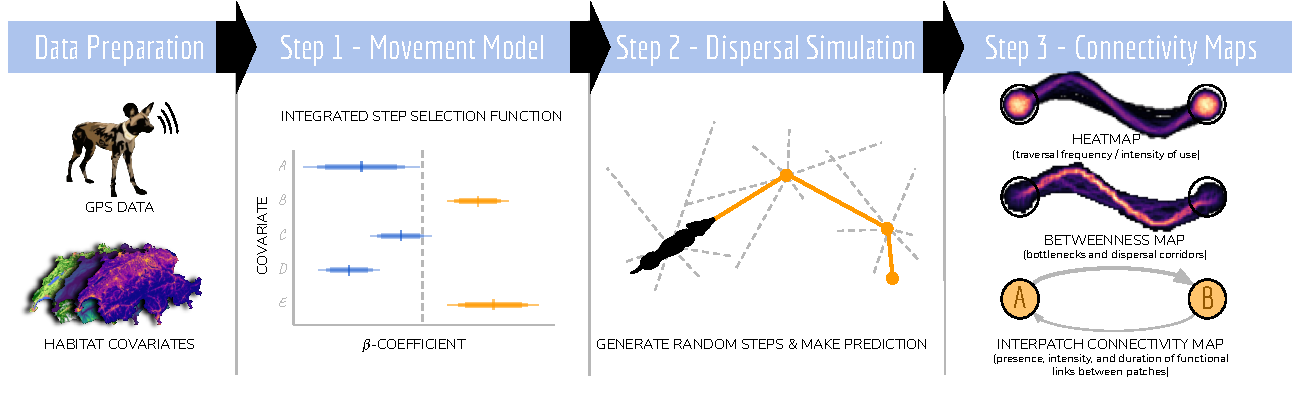
\includegraphics[width = \textwidth]{99_GraphicalAbstract.pdf}
    \caption{Flowchart of the simulation-based connectivity analysis. First, GPS
    data and habitat covariates must be collected. The combined data is then
    analyzed using an integrated step selection model (step 1). The parametrized
    model is then treated as an individual-based movement model and used to
    simulate dispersal trajectories (step 2). Ultimately, simulated trajectories
    are translated into a set of maps that are pertinent to landscape
    connectivity (step 3). This includes a heatmap, indicating the traversal
    frequency across each spatial unit of the study area, a betweenness map,
    highlighting movement corridors and bottlenecks, and, finally, an
    inter-patch connectivity map, where the frequency of connections and their
    average duration can be depicted.}
    \label{GraphicalAbstract}
  \end{center}
\end{figure}

\section{Methods}
\subsection{Case Study}
\subsubsection{GPS Data}
We applied the three step approach presented in \Cref{GraphicalAbstract} to GPS
movement data from 16 dispersing African wild dog coalitions (7 female and 9
male coalitions). This data has been collected between 2011 and 2019 from a
free-ranging wild dog population in northern Botswana. During dispersal, GPS
collars recorded a fix every 4 hours and regularly transmitted data over the
Iridium satellite system. To ensure comparable time intervals between GPS fixes,
we removed any fixes that were not successfully obtained at the desired 4-hour
schedule (allowing for a tolerance of \( \pm \) 15 minutes). To prepare the data
for step-selection analysis, we converted the fixes (n = 4'169) into steps,
where each step represented the straight-line movement between two consecutive
GPS fixes \citep{Turchin.1998}. We only considered steps with equal
step-durations (i.e. 4 hours) for further analysis. We will refer to these steps
as ``realized steps''. We did not differentiate between sexes, for previous
research found little differences between sexes during dispersal
\citep{Woodroffe.2019, Cozzi.2020}. Additional details on the data collection
and preparation can be found in \cite{Cozzi.2020} and \cite{Hofmann.2021}.

% To delineate periods of dispersal, we determined the exact timing of emigration
% from the natal pack and settlement in a new territory using direct field
% observations and through visual inspection of the net squared displacement (NSD)
% metric. The NSD metric measures the squared Euclidean distance of a GPS
% relocation to a reference point \citep{Borger.2012}, which we set to the center
% of the territory of each dispersers' natal pack. Thus, dispersal was deemed to
% have started once an individual left its natal territory and ended once the NSD
% metric remained constant, indicating settlement. Because behavior during
% dispersal is more pertinent to landscape connectivity than behavior during
% residence \citep{Elliot.2014, Abrahms.2017}, we only considered data collected
% during dispersal for our analysis.

\subsubsection{Study Area}
Our simulation of dispersal trajectories and assessment of connectivity spanned
across the entire Kavango-Zambezi Transfrontier Conservation Area (KAZA-TFCA,
\Cref{StudyArea}a and b) and encompassed a rectangular extent of roughly 1.3
Mio. km\textsuperscript{2}. With an area of 520'000 km\textsuperscript{2}, the
KAZA-TFCA is the world's largest transboundary conservation area and comprises
parts of Angola, Botswana, Namibia, Zimbabwe, and Zambia, thus hosting a rich
diversity of landscapes, ranging from savannah to grassland and from dry to
moist woodland habitats. In its center lies the Okavango Delta, a dominant
hydro-geographical feature and the world's largest flood-pulsing inland delta.
Large portions of the KAZA-TFCA are formally protected in the form of national
parks (NPs) or other protected areas, yet a considerable portion of the
landscape remains human-dominated (e.g. roads, agricultural sites, and
settlements).

\begin{figure}[h]
  \begin{center}
    \begin{tikzpicture}
        \node[anchor=south west,inner sep=0] (image) at (0,0,0) {
        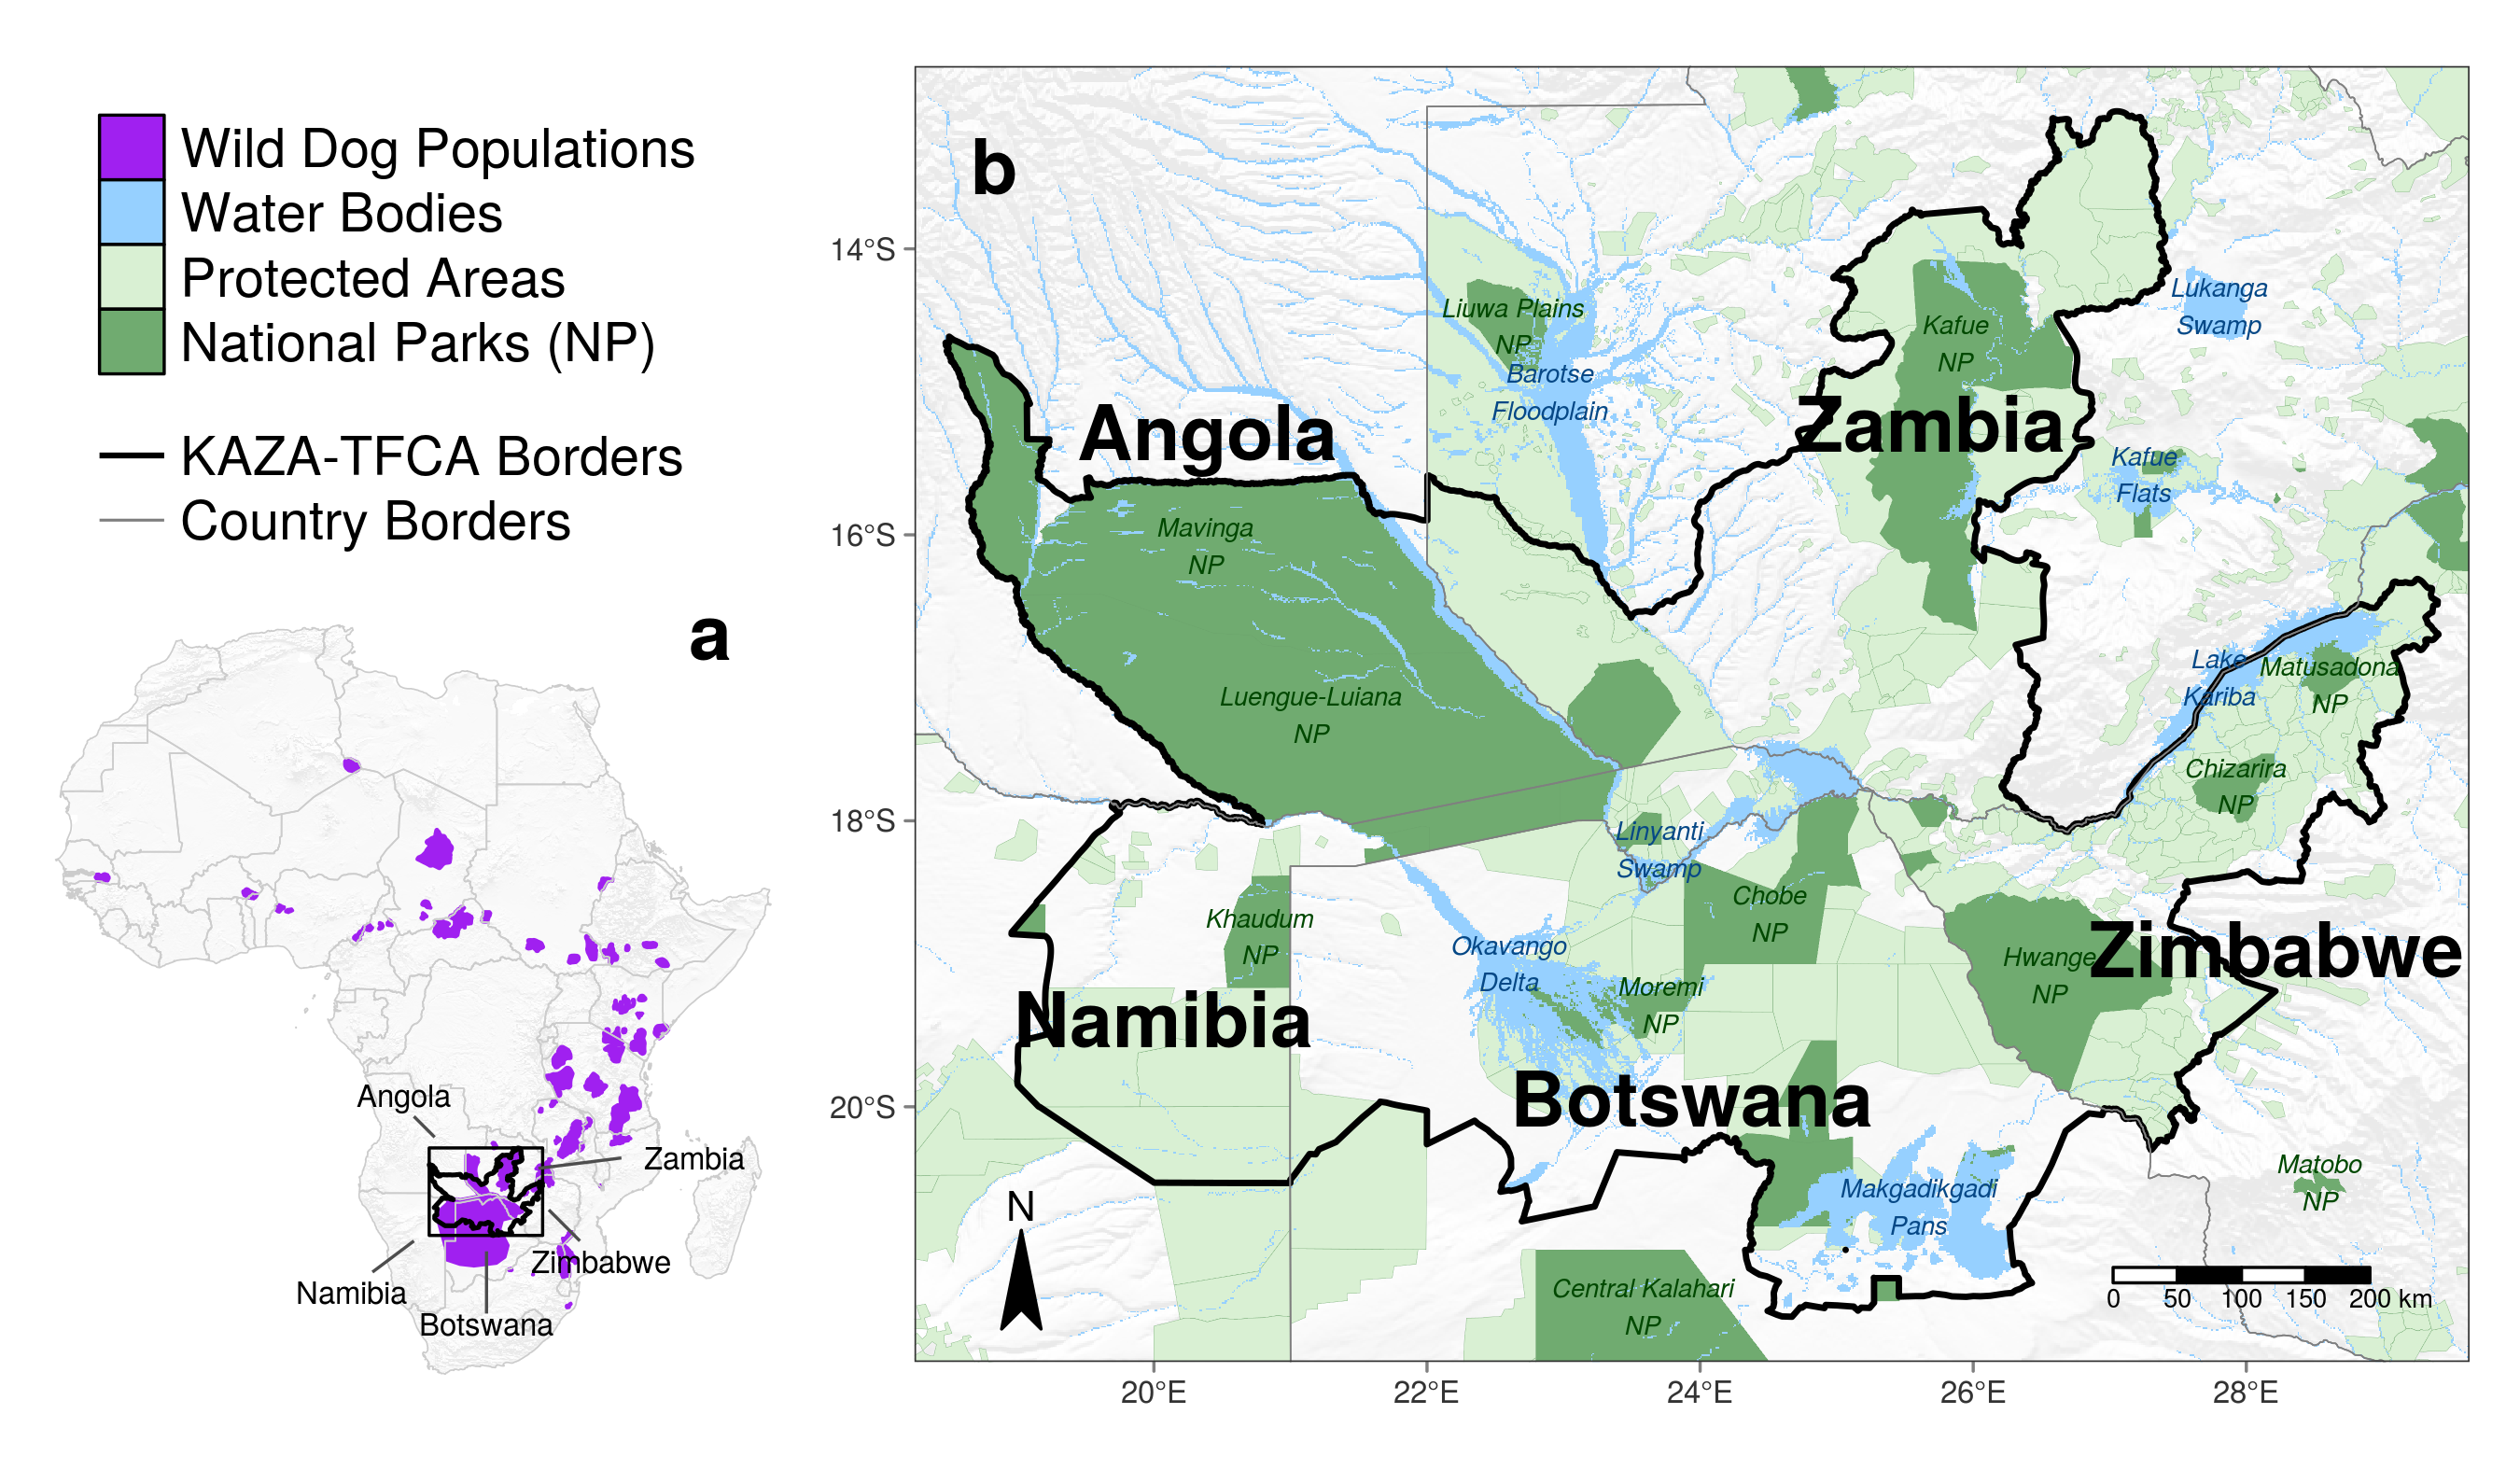
\includegraphics[width=\textwidth]{99_StudyArea.png}
        };
        \begin{scope}[x={(image.south east)},y={(image.north west)}]
            % % next four lines will help you to locate the point needed by forming a grid.
            % % comment these four lines in the final picture.
            % \draw[help lines,xstep=.1,ystep=.1] (0,0) grid (1,1);
            % \draw[help lines,xstep=.05,ystep=.05] (0,0) grid (1,1);
            % \foreach \x in {0,1,...,9} { \node [anchor=north] at (\x/10,0) {0.\x}; }
            % \foreach \y in {0,1,...,9} { \node [anchor=east] at (0,\y/10) {0.\y};}
            % % upto here
            \draw[densely dotted, blue] (0.169, 0.222) -- (0.364, 0.955);
            \draw[densely dotted, blue] (0.169, 0.157) -- (0.364, 0.074);
        \end{scope}
    \end{tikzpicture}
    \caption{Illustration of the study area in southern Africa. (a) The study
    area was confined by a bounding box spanning the entire KAZA-TFCA which
    comprises parts of Angola, Namibia, Botswana, Zimbabwe, and Zambia. Data on
    remaining wild dog populations (orange) has been sourced from
    \cite{Woodroffe.2012}. (b) The KAZA-TFCA represents the world's largest
    terrestrial transfrontier conservation area and covers a total area of
    520'000 km\textsuperscript{2}. Its main purpose is to re-establish
    connectivity between already-existing NPs (dark green) and other protected
    areas (light green).}
    \label{StudyArea}
  \end{center}
\end{figure}

\subsubsection{Habitat Covariates}
We represented the physical landscape in our study area by the habitat
covariates \textsf{water-cover, distance-to-water, woodland-cover,
shrub/grassland-cover, and human-influence}. To render the seasonal dynamics of
water-cover for the extent of the Okavango Delta, we applied an algorithm that
enabled us to obtain weekly updated raster-layers for \textsf{water-cover} and
\textsf{distance-to-water} from MODIS satellite imagery \citep{Wolski.2017,
Hofmann.2021}. This algorithm is now implemented in the {\tt floodmapr} package
(available on GitHub; \url{https://github.com/DavidDHofmann/floodmapr}). To
ensure a consistent resolution across habitat covariates, we coarsened or
interpolated all layers to a resolution of 250 m x 250 m. A detailed description
of how we prepared each habitat covariate is provided in \cite{Hofmann.2021}.

We performed all data preparations, spatial computations, and statistical
analysis in {\tt R}, version 3.6.6 \citep{R.2020}. Some helper functions were
written in {\tt C++} and imported into {\tt R} using the {\tt Rcpp} package
\citep{Eddelbuettel.2011, Eddelbuettel.2013, Eddelbuettel.2018}.

\subsection{Step 1 - Movement Model}
We combined the collected GPS data with habitat covariates and used ISSFs
\citep{Avgar.2016} to parametrize a mechanistic movement model. More
specifically, we paired each realized step with a set of 24 randomly generated
alternative steps. A realized and its 24 random steps together formed a stratum
that received a unique identifier. As suggested by \cite{Avgar.2016}, we
generated random steps by sampling random turning angles from a uniform
distribution (\(-\pi, +\pi\)) and step lengths from a gamma distribution that
was fitted to realized steps (scale \(\theta\) = 6'308 and shape \(k\) = 0.37).
Note that our approach of sampling turning angles from a uniform distribution
does not imply that we assume uniform turning angles, as we will account for
directionality later in the model \citep{Avgar.2016, Fieberg.2021}.

Along each realized and random step, we extracted values from underlying habitat
covariate layers and we computed averages of each covariate along the steps.
Besides extracting \textit{habitat covariates}, we also computed movement
metrics that we used as \textit{movement covariates} in the ISSF models
\citep{Avgar.2016, Fieberg.2021}. Specifically, we computed the step length
(\textsf{sl}), its natural logarithm (\textsf{log(sl)}), and the cosine of the
relative turning angle (\textsf{cos(ta)}), which is a measure of directionality
\citep{Turchin.1998}, for each step. Because wild dog activity is low during the
hot midday hours \citep{Cozzi.2012}, we additionally created the variable
\textsf{LowActivity}, indicating whether a step was realized during periods of
low wild dog activity (09:00 to 17:00 local time) or high wild dog activity
(17:00 to 09:00 local time). To facilitate model convergence, we standardized
all continuous covariates to a mean of zero and a standard deviation of one.
Correlations among covariates were low (\(|r| < 0.6\); \citealp{Latham.2011}),
so we retained all of them for modeling.

To contrast realized steps (scored 1) and random steps (scored 0), we assumed
that animals assigned a selection score \(w(x)\) to each step (\ref{EQ1};
\citealp{Fortin.2005}), where \(w(x)\) depended on the step's associated
covariates (\(x_1, x_2, ..., x_n\)) and on the animal's relative selection
strengths \citep{Avgar.2017} towards these covariates (\(\beta_1, \beta_2,
..., \beta_n\)):

\begin{equation}
\label{EQ1}
  w(x) = exp(\beta_1 x_1 + \beta_2 x_2 + ... + \beta_n x_n)
\end{equation}

\noindent The probability of a step \(i\) being realized was then contingent on
the step's selection score, as well as on the selection scores of all other step
in the same stratum:

\begin{equation}
\label{EQ2}
  P(Y_{i} = 1 | Y_{1} + Y_{2} + ... + Y_{i} = 1) =
  \frac{w(x_{i})}{w(x_{1}) + w(x_{2}) + ... + w(x_{i})}
\end{equation}

\noindent To estimate relative selection strenghts (i.e. the
\(\beta\)-coefficients), we used mixed effects conditional logistic regression
analysis, implemented through the r-package {\tt glmmTMB} \citep{Brooks.2017}.
The implementation of conditional logistic regression has been proposed by
\cite{Muff.2020} and allows to model random slopes. The method requires to fix
the variance of the stratum specific intercept to a large value, so we fixed it
to an arbitrary high value of \(10 ^ 6\) and used disperser identity to model
random slopes for all covariates.

Our movement model was based on a habitat selection model that was previously
developed for dispersing wild dogs (hereafter referred to as \textit{base
model}, \citealp{Hofmann.2021}). In the base model, no interactions among
habitat covariates and movement covariates were considered, so we here expanded
the model and allowed for such interactions, acknowledging that movement
preferences during dispersal could depend on habitat conditions (details in
Appendix A1). To determine the most parsimonious movement model among model
candidates, we ran stepwise forward model selection based on Akaike's
Information Criterion (AIC, \citealp{Burnham.2002}). More specifically, we
started with the base model and iteratively increased model complexity by adding
all possible interactions between movement and habitat covariates. Given that
the focus of our analysis lied on predicting dispersal patterns and all model
candidates were biologically intuitive, we deemed the use of model selection
appropriate. However, caution should be employed if causal relationships are of
interest, as model selection may lead to biased parameter estimate
\citep{Whittingham.2006}. We validated the predictive power of the most
parsimonious model using k-fold cross-validation for case-control studies as
described in \cite{Fortin.2009}. This validation attests significant prediction
ability to the movement model if the model outperforms a random guess and
systematically assigns low ranks (high selection scores) to observed steps
(details in Appendix A2).

\subsection{Step 2 - Dispersal Simulation}
We used the most parsimonious movement model to simulate individual dispersal
trajectories across the study area. The simulation of a dispersal trajectory
resembled an ``inverted'' ISSF and was set up as follows. (1) We defined a
source point and assumed a random initial orientation of the simulated animal.
(2) Starting from the source point, we generated 25 random steps by sampling
turning angles from a uniform distribution (\(-\pi, +\pi\)) and step lengths
from our fitted gamma distribution. (3) Along each random step, we extracted and
averaged values from the habitat covariate layers and we computed the movement
metrics \textsf{sl}, \textsf{log(sl)}, and \textsf{cos(ta)}. To ensure
compatible scales with the fitted movement model, we standardized covariate
values using means and standard deviations from the empirical data. (4) We
applied the parametrized movement model to predict the selection score \(w(x)\)
for each step using \ref{EQ1} and we converted predicted scores into
probabilities using \ref{EQ2}. (5) We randomly sampled one of the generated
random steps based on assigned probabilities and determined the animal's new
position. We repeated steps (2) to (5) until 2,000 steps were realized and we
repeated the simulation until a total of 80'000 dispersal trajectories was
reached.

As source points for the simulations, we distributed 50,000 points at random
locations inside protected areas that were large enough to host an average size
wild dog home range (i.e. \(>\) 700 km\textsuperscript{2};
\citealp{Pomilia.2015}). We placed another 30,000 points randomly inside the
buffer zone, mimicking potential immigration into the study area (Figure S1).

To mitigate edge effects and to deal with random steps leaving the study area,
we followed \cite{Koen.2010} and artificially expanded all covariate layers by a
100 km wide buffer zone. Within the buffer zone, we randomized covariate values
by resampling values from the original covariate layers. Through this buffer
zone, simulated dispersers were able to leave and re-enter the main study area.
In cases where random steps crossed the outer border of this buffer zone, we
resampled steps until they fully lied within the buffer zone, essentially
forcing simulated individuals to remain within the expanded study area.

To ensure reliable connectivity estimates, we determined the number of simulated
dispersal trajectories required to reach a ``steady state''. For this purpose,
we distributed 1,000 rectangular ``checkpoints'', each with an arbitrary extent
of 5 km x 5 km, at random coordinates within the study area (excluding the
buffer). We then determined the relative frequency at which each checkpoint was
traversed by simulated dispersal trajectories (hereafter referred to as relative
traversal frequency) as we gradually increased the number of simulated
trajectories from 1 to 50,000. To assess variability in the relative traversal
frequency, we repeatedly subsampled 100 times from all 50'000 trajectories and
computed the mean traversal frequency across replicates, as well as its 95\%
prediction-interval for each checkpoint. We considered connectivity to have
reached a steady state once the width of the prediction-interval dropped below a
value of 0.01 for all checkpoints.

\subsection{Step 3 - Connectivity Maps}
\subsubsection{Heatmap}
To identify dispersal hotspots within the study area, we created a heatmap
indicating the absolute frequency at which different areas were traversed by
simulated dispersal trajectories (e.g. \citealp{Hauenstein.2019, Zeller.2020}).
Specifically, we rasterized all simulated trajectories onto a raster with 1 km x
1 km resolution and tallied resulting layers into a single map. This procedure
ensured that every trajectory was only counted once, even if it traversed the
same raster-cell multiple times, thus reducing potential biases caused by
individuals that were surrounded by unfavorable habitat and ``moved in
circles''. To achieve high performance rasterization, we used the R-package {\tt
terra} \citep{Hijmans.2021b}.

\subsubsection{Betweenness Map}
To pinpoint movement corridors and bottlenecks, we converted simulated
trajectories into a network and calculated betweenness scores for all
raster-cells in the study area \citep{BastilleRousseau.2018}. Betweenness is a
pertinent metric for connectivity as it measures how often a specific
network-node (in our case a raster-cell) lies on a shortest path between any
other pair of nodes \citep{BastilleRousseau.2018}. To convert simulated
trajectories into a network, we followed \cite{BastilleRousseau.2018} and
overlaid the study area (including the buffer) with a raster containing 2.5 km x
2.5 km raster-cells, where the center of each raster-cell served as node in the
final network. To identify edges (i.e. connections) between the nodes, we used
the simulated trajectories and determined all transitions occurring from one
cell to another, as well as the frequency at which those transitions occurred
(see also Appendix A4). This resulted in an edge-list that we translated into a
weighted network using the r-package {\tt igraph} \citep{Gabor.2006}. The final
weight of each edge was determined by the frequency of transitions, yet because
{\tt igraph} handles edge weights (\(\omega\)) as costs, we inverted the
traversal-frequency through each raster-cell by applying \(\omega =
\frac{mean(Traversal Frequency)}{Traversal Frequency_i}\). Consequently,
regularly used edges received small weights (i.e. low costs) and vice versa. We
used the weighted network to calculate betweenness scores for all network nodes.

\subsubsection{Inter-Patch Connectivity Map}
To examine the presence and intensity of functional links (i.e. connections)
between patches within the study area, we calculated inter-patch connectivity
(e.g. \citealp{Gustafson.1996}, \citealp{Kanagaraj.2013}). For this, we computed
the relative frequency at which dispersers originating from one patch
successfully moved into another patch. We considered movements between patches
as successful if an individual's dispersal trajectory originating from the
source patch intersected with the target patch at least once. For each
trajectory we also recorded the number of steps required to reach the first
intersection with the respective patch, allowing us to compute the average
dispersal durations from one patch to another. In summary, we determined
\textit{if} and \textit{how often} dispersers moved between certain patches, as
well as \textit{how long} individuals had to move to make these connections. In
our case study, we used NPs as patches to determine inter-patch connectivity,
hence we'll use the terms interchangeably from here on. The decision to focus on
NPs was purely out of simplicity and should not imply that dispersal between
other areas is impossible.

\subsubsection{Validation}
To validate our predictions of connectivity, we utilized additional dispersal
data that was collected on eight dispersing coalitions between the years 2019
and 2022 (totalling to 2'668 GPS locations). We used path selection analysis
(PSF, \citealp{Cushman.2010}) to assess if observed dispersal trajectories
followed areas of high predicted connectivity. Similar to SSF, PSF enables to
detect selection for certain features by comparing observed paths to randomly
generated paths. Here, we paired each observed path with 50 random paths that we
generated by randomly rotating and shifting observed paths by a random angle
\(\alpha \sim U(-\pi, +\pi)\) and a random distance \(d \sim U(0 \) km, \(50\)
km\(\)). Along each path, we then extracted connectivity values from the heatmap
(see above) generated after 68, 125, 250, 500, and 2'000 simulated steps,
respectively. Finally, we ran conditional logistic regression to contrast
observed and random paths. In case of systematic selection for high-connectivity
areas, the regression coefficients from the corresponding conditional logistic
regression model should be positive.

\section{Results}
% \subsection{Movement Model}
The most parsimonious movement model consisted of movement covariates, habitat
covariates, as well as several of their interactions, thus suggesting that
movement behavior during dispersal depended on habitat conditions
(\Cref{MovementModel}a, Table S1 and Table S2). Although multiple models
received an AIC weight \(>\) 0 (Table S1), we only considered results from the
most parsimonious model for simplicity. This decision only marginally influenced
subsequent steps as all models with positive AIC weights retained similar
covariates (Table S1). The k-fold cross-validation showed that the final model
substantially outperformed a random guess and provided reliable predictions
(i.e. confidence intervals of \(\bar{r}_{s, realized}\) and \(\bar{r}_{s,
random}\) did not overlap). Moreover, the model correctly assigned high
selection scores to realized steps (\Cref{MovementModel}b), indicating a good
fit between predictions and observations. As can be taken from the Spearman rank
correlation coefficient, the inclusion of several interactions between movement
and habitat covariates significantly improved model performance (\(\bar{r}_{s,
realized} = -0.65; 95\%-CI = [-0.67, -0.64]\)), compared to the base model
(\(\bar{r}_{s, realized} = -0.55; 95\%-CI = [-0.57, -0.52]\);
\citealp{Hofmann.2021}). Our validation of the resulting connectivity maps using
independent dispersal data showed that dispersers preferentially followed areas
of high predicted connectivity, as coefficients from the PSF models were all
significantly greater than zero (\Cref{MovementModel}c). The movement model thus
successfully predicted functional connectivity.

Plots that aid with the interpretation of the most parsimonious movement model
are provided in Figure S3 and suggest that, under average conditions, dispersing
wild dogs avoided moving through water, woodlands, and areas dominated by
humans, but preferred moving across shrublands or grasslands
(\Cref{MovementModel}a). Dispersers realized shorter steps (indicating slower
movements) in areas covered by water or woodland, while realizing larger steps
in areas dominated by shrubs or grass (\Cref{MovementModel}a). We found a
particularly large effect for the variable \textsf{LowActivity}, suggesting that
dispersing wild dogs moved substantially faster during twilight and at night
(i.e. between 17:00 and 09:00 o'clock; \Cref{MovementModel}a). Although
dispersers revealed a preference for directional movements (i.e. low turning
angles), especially when moving quickly, they did less so in proximity to humans
or water, resulting in more tortuous movements in such areas
(\Cref{MovementModel}a).

\begin{figure}
  \begin{center}
    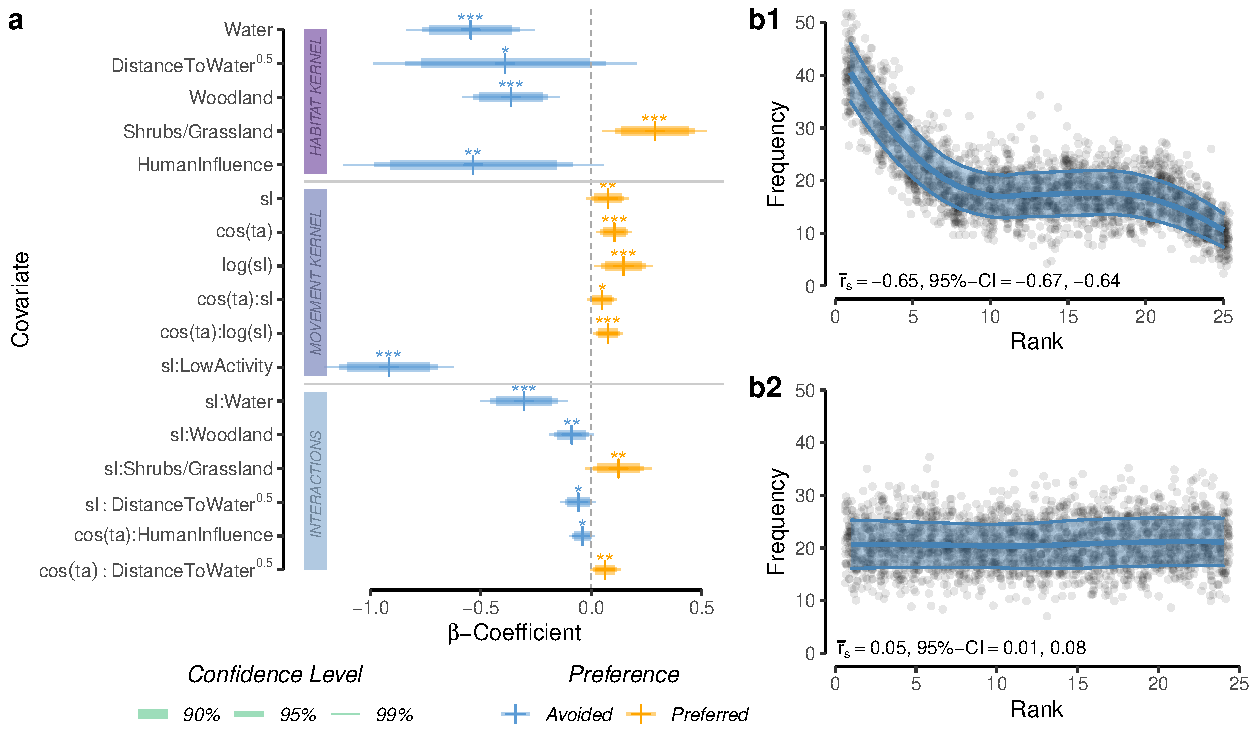
\includegraphics[width=\textwidth]{99_MovementModel}
    \caption{(a) Most parsimonious movement model for dispersing wild dogs. The
    model comprises a habitat kernel, a movement kernel, as well as their
    interactions. The horizontal line segments delineate the 90\%, 95\%, and
    99\% confidence-intervals for the respective \(\beta\)-coefficients.
    Significance codes: * \(p < 0.10\), ** \(p < 0.05\), *** \(p < 0.01\). (b)
    Results from the k-fold cross validation procedure. Subfigure b1 shows rank
    frequencies of realized steps according to model predictions with known
    preferences, whereas subfigure b2 shows rank frequencies of realized steps
    when assuming random preferences. The blue ribbon shows the prediction
    interval around a loess smoothing regression that we fitted to ease the
    interpretation of the plots. The significant correlation between rank and
    associated frequency in (b1) highlights that the most parsimonious model
    successfully outperformed a random guess (b2) and frequently assigned low
    ranks (i.e. high selection scores) to realized steps but only rarely high
    ranks (i.e. low selection scores). (c) Results from the PSF analysis using
    independent dispersal data show that dispersers preferrably moved through
    areas where our heatmaps predicted high connectivity. Results are shown for
    heatmaps realized after 68, 125, 250, 500, and 2'000 simulated steps,
    respectively.}
    \label{MovementModel}
  \end{center}
\end{figure}

\subsection{Dispersal Simulation}
Dispersal simulations based on the most parsimonious movement model proved
useful for assessing landscape connectivity. Of the 50,000 simulated dispersal
trajectories that originated from the main study area, only 4.5\% reached a map
boundary, suggesting that we successfully mitigated biases from boundary
effects. Moreover, our examination of the relative traversal frequency across
all checkpoints showed that the relative traversal frequency reached a steady
state after 10,500 simulated dispersal trajectories (Figure S4). Although
variability in the relative traversal frequency kept decreasing as we increased
the number of simulated dispersers, the marginal benefit of simulating
additional trajectories diminished quickly (Figure S4).

\subsection{Heatmap}
The heatmap (\Cref{Heatmap}), which resulted from the summation of all simulated
dispersal trajectories, allowed us to pinpoint areas that were frequently
visited and enabled us to compare areas inside and outside the KAZA-TFCA borders
with respect to the intensity at which they were used for dispersal. For
instance, we could deduct that areas inside the KAZA-TFCA were frequently
traversed by dispersers (median traversal frequency inside KAZA-TFCA = 166, IQR
= 274, Figure S7a), whereas areas beyond the KAZA-TFCA boundary were
comparatively rarely visited (median traversal frequency outside KAZA-TFCA = 61,
IQR = 133, Figure S7a). Most notably, the region in northern Botswana south of
the Linyanti swamp appeared to serve as highly frequented dispersal hotspot
(median traversal frequency = 987, IQR = 558). Aside from revealing movement
hotspots, the heatmap also provided information on areas that appeared to hinder
movement. For example, extensive water bodies, such as the Okavango Delta, the
Makgadikgadi Pan, and the Linyanti swamp, substantially restricted dispersal
movements and limited realized connectivity inside the KAZA-TFCA. Similarly, the
landscapes of Zambia and Zimbabwe were only rarely used for dispersal, even
within the KAZA-TFCA boundaries (Figure S8a). Despite the fact that the heatmap
improved our understanding of the frequency at which areas were traversed by
simulated dispersers, it seemed impractical to pinpoint dispersal corridors.

\begin{figure}
  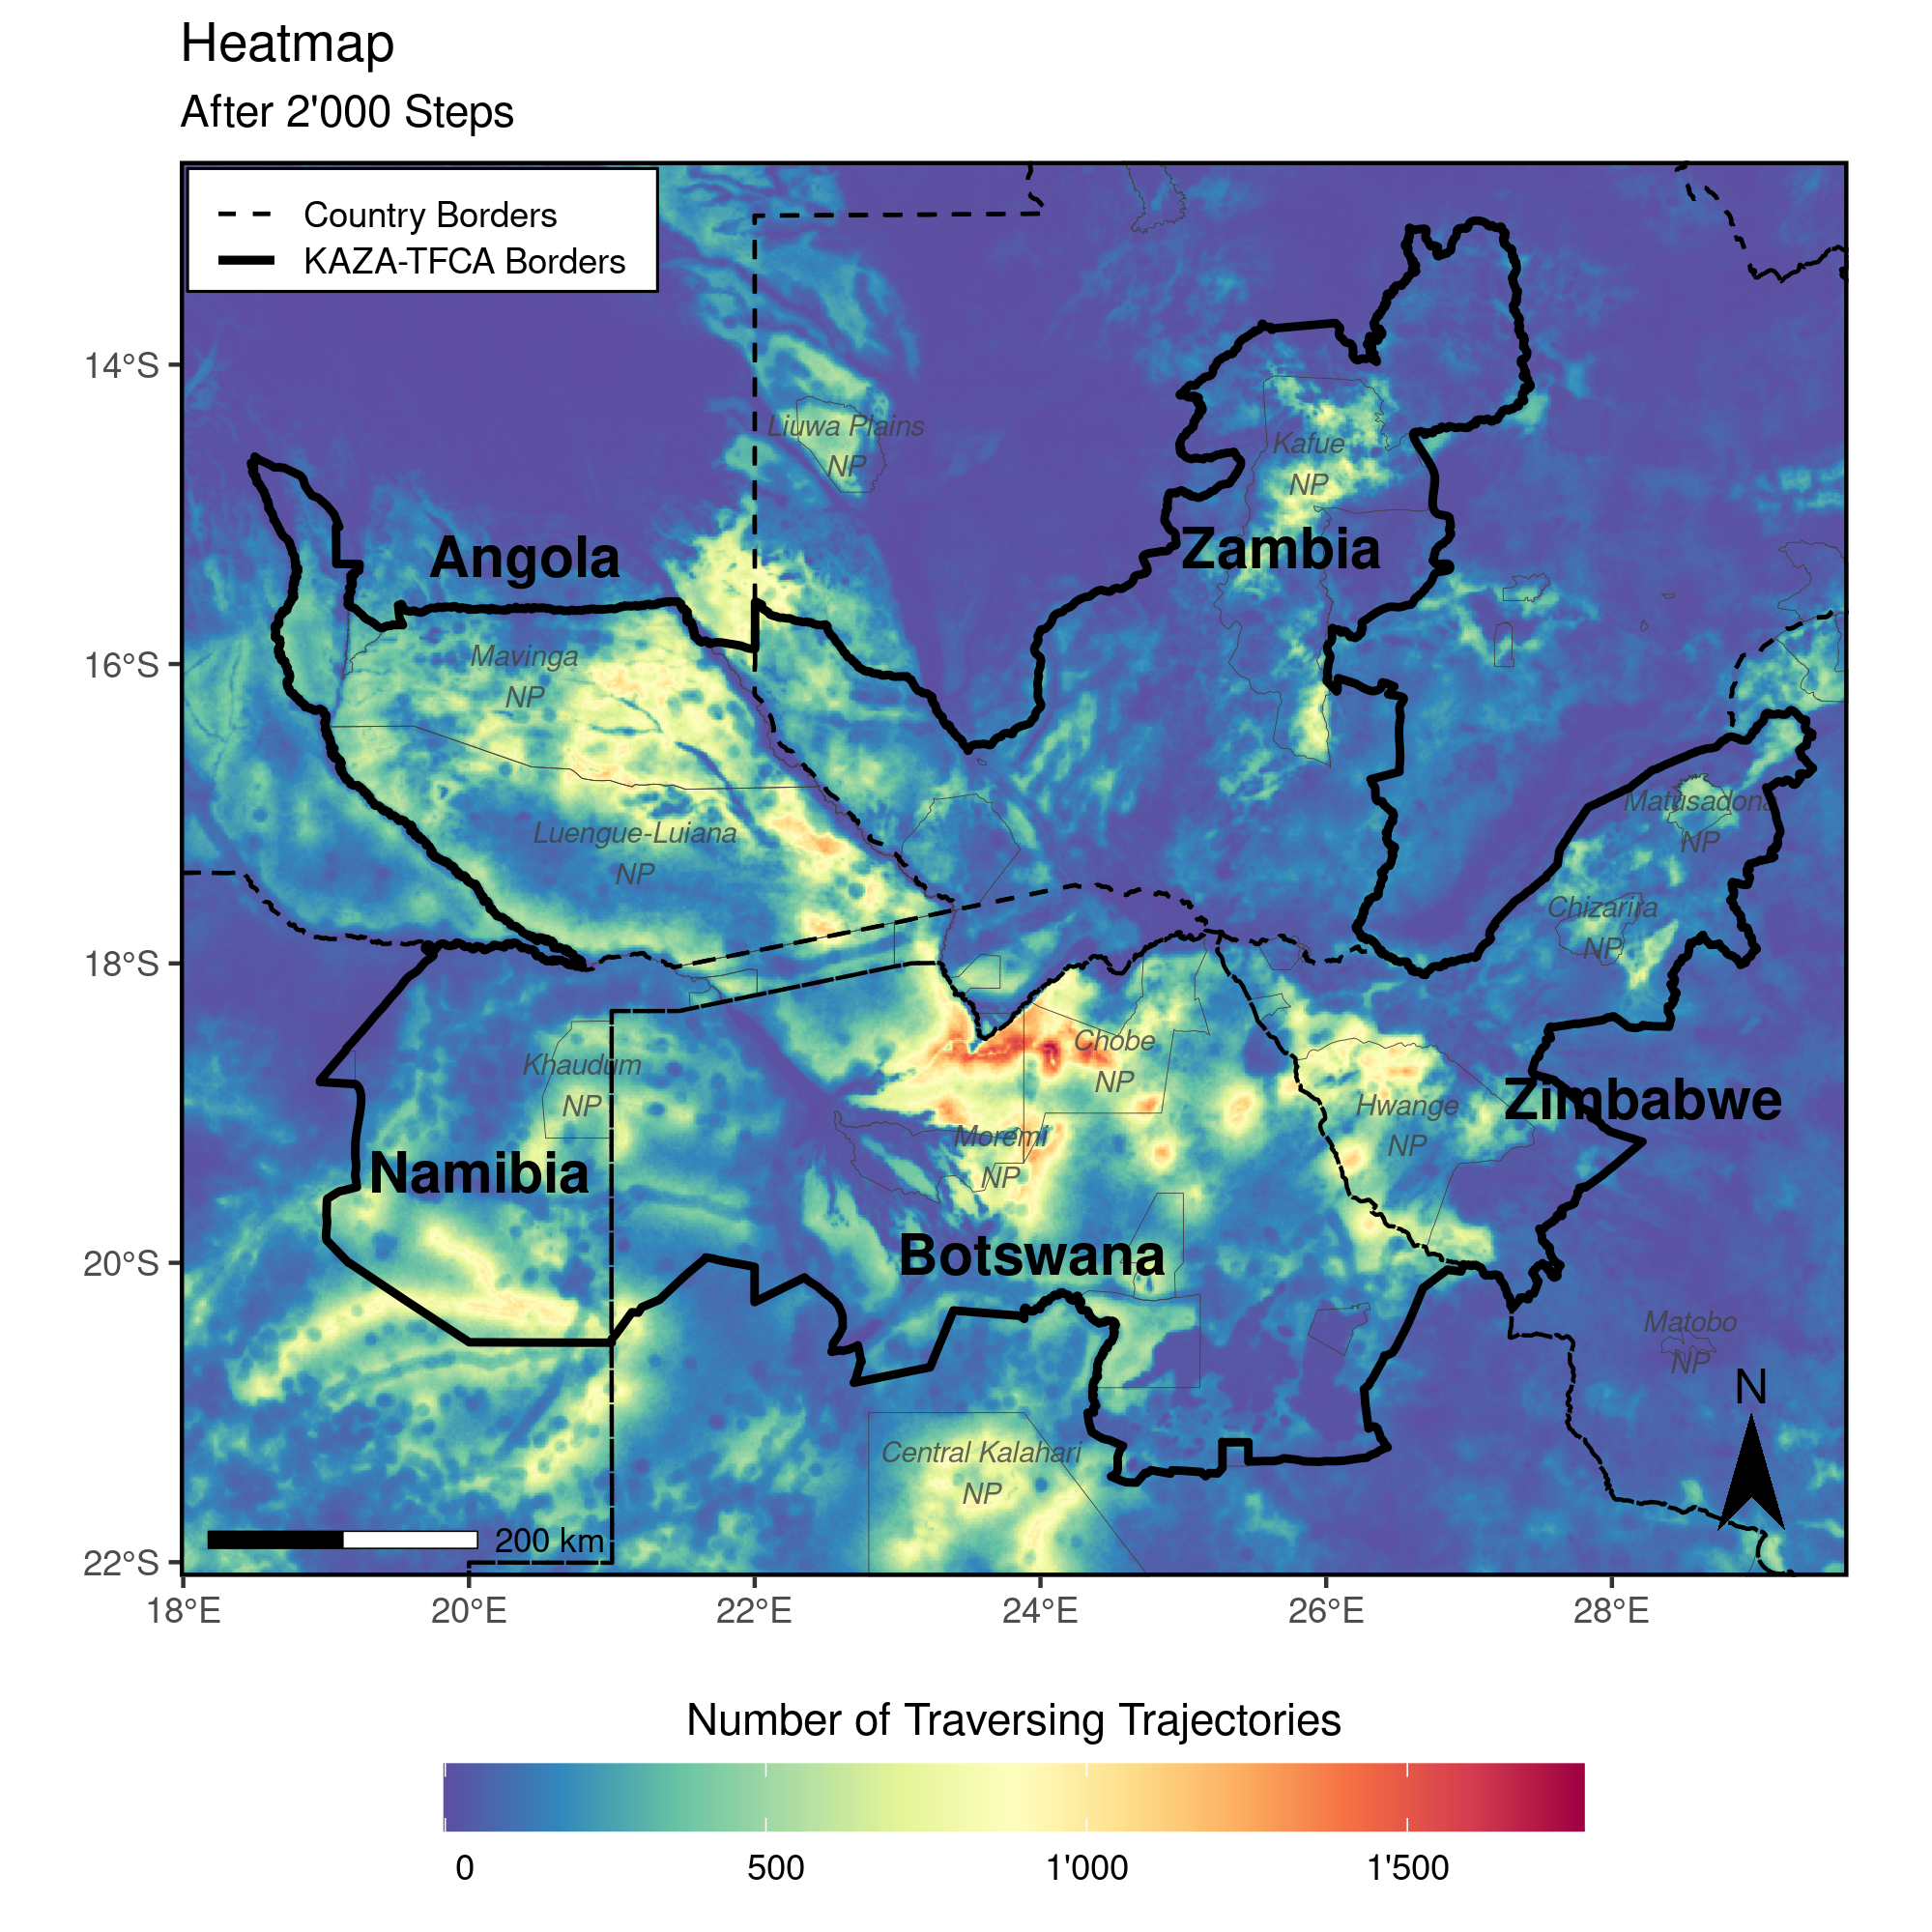
\includegraphics[width=\textwidth]{99_Heatmap.png}
  \caption{Heatmap showing traversal frequencies of 80'000 simulated dispersers
  moving 2'000 steps across the KAZA-TFCA. Simulations were based on an
  integrated step-selection model that we fitted to the movement data of
  dispersing African wild dogs. To generate the heatmap, we rasterized and
  tallied all simulated trajectories. Consequently, the map highlights areas
  that are frequently traversed. For spatial reference we plotted a few selected
  NPs (dark gray). Additional heatmaps showing the traversal frequency when
  individuals move fewer than 2'000 steps are provided in Figure S5.}
  \label{Heatmap}
\end{figure}

\subsection{Betweenness}
The betweenness map (\Cref{Betweenness}) revealed several distinct dispersal
corridors that run across the study area. In comparison to the heatmap, the
betweenness map was less biased towards areas with many dispersers and
pronounced narrower, more linear routes that were used by simulated individuals
to move between regions. Again, northern Botswana emerged as a wild dog
dispersal corridor that connected more remote regions in the study area. Towards
east, the extension of this corridor ran through Chobe NP into Hwange NP. From
there, a further extension connected to Matusadona NP in Zimbabwe. Northwest of
the Linyanti ecosystem, a major corridor expanded into Angola, where it split
and finally traversed over a long stretch of unprotected area into Zambia's
Kafue NP. Several additional corridors with lower betweenness scores emerged,
yet most of them ran within the KAZA-TFCA boundaries (median betweenness inside
KAZA-TFCA = 6.947 \(\times\) 10\textsuperscript{6}, IQR = 54.311 \(\times\)
10\textsuperscript{6}, Figure S7b). Consequently, only few corridors directly
linked the peripheral regions of the KAZA-TFCA and passed through unprotected
areas outside its borders (mean betweenness outside KAZA-TFCA = 2.685 \(\times\)
10\textsuperscript{6}, IQR = 9.891 \(\times\) 10\textsuperscript{6}, Figure
S7b).

%  9 2000  Betweenness Inside KAZA-TFCA  6946817.   54311358.
% 10 2000  Betweenness Outside KAZA-TFCA 2685174.    9890504.

\begin{figure}
  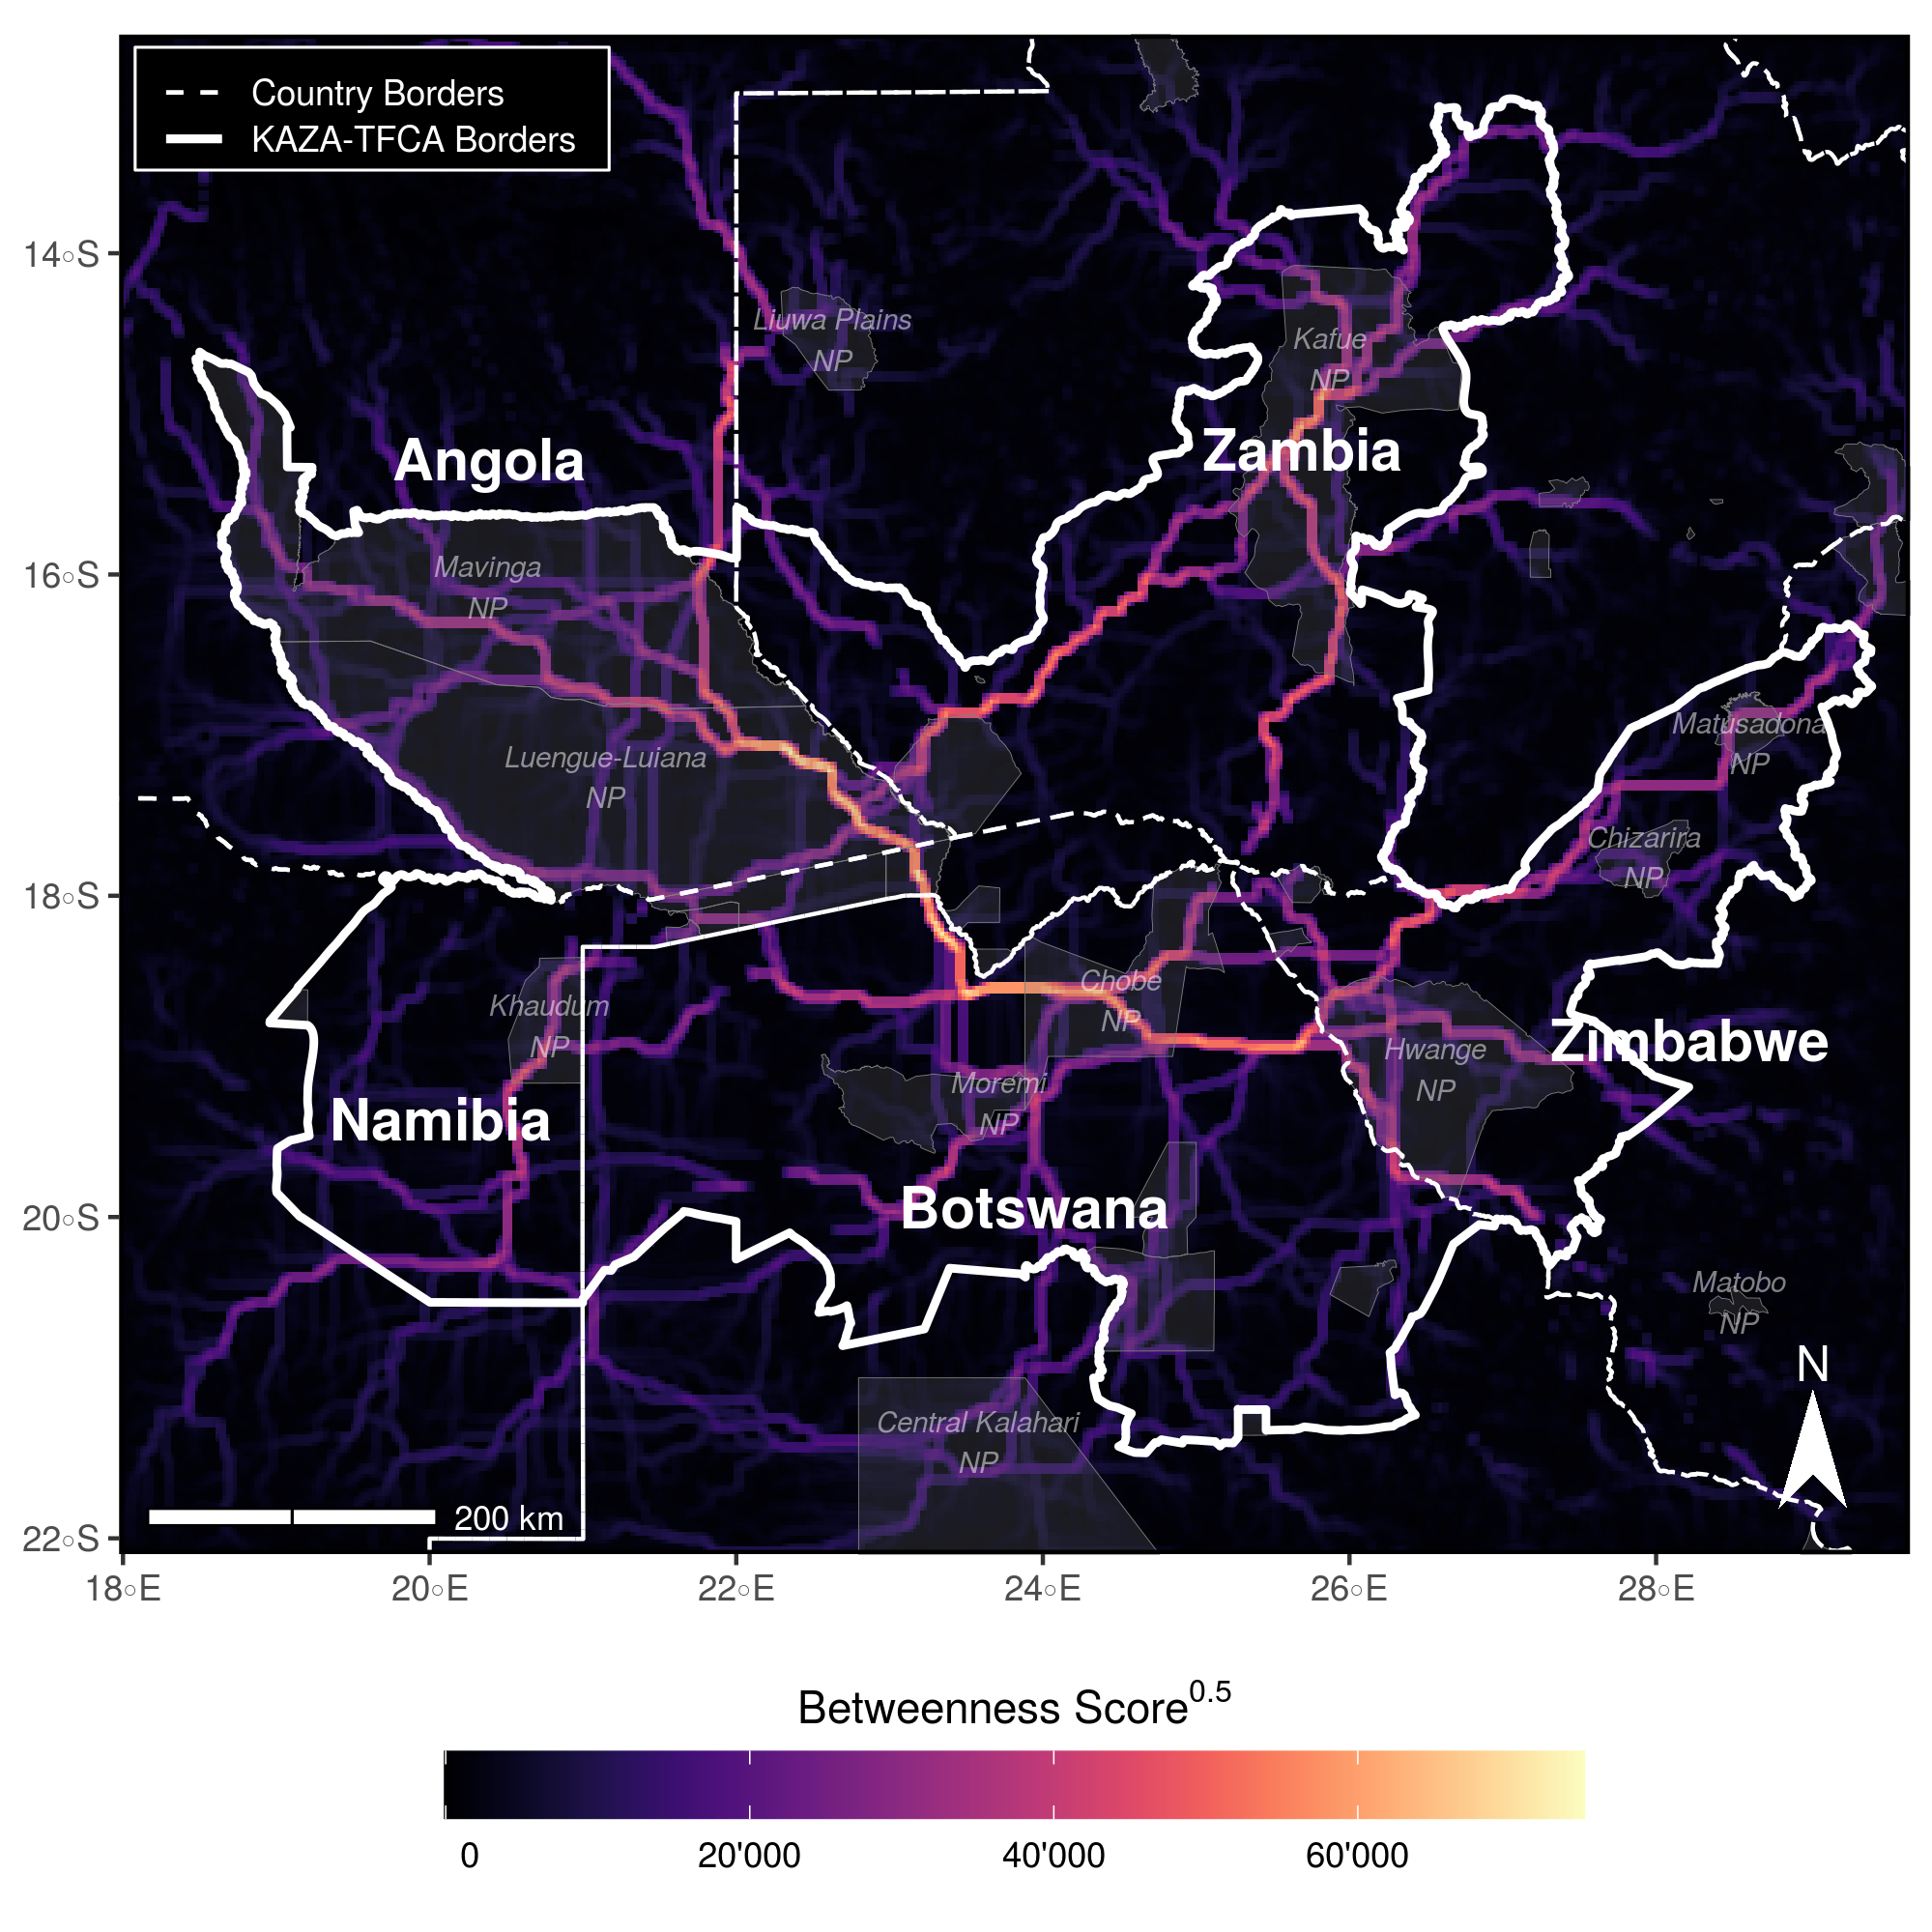
\includegraphics[width=\textwidth]{99_Betweenness.png}
  \caption{Map of betweenness scores, highlighting distinct dispersal corridors
  and potential bottlenecks across the extent of the KAZA-TFCA. Betweenness
  measures the number of shortest paths traversing through each node
  (raster-cell). Hence, a high betweenness score indicates that the respective
  area is exceptionally important for connecting different regions in the study
  area. The metric is therefore useful to pinpoint discrete movement corridors
  \citep{BastilleRousseau.2018}. Note that we square-rooted betweenness scores
  to improve visibility of corridors with comparably low scores. Additional
  betweenness maps showing betweenness scores when individuals move fewer than
  2'000 steps are provided in Figure S6.}
  \label{Betweenness}
\end{figure}

\subsection{Inter-Patch Connectivity}
The inter-patch connectivity map showed that the relative frequency at which
simulated dispersal trajectories moved from one patch to another varied, as did
the average dispersal duration between patches (\Cref{InterpatchConnectivity}).
The map thereby completed the picture on connectivity and provided valuable
insights into the frequency and duration of connections between patches. For
some patches, we also detected imbalances between the number of incoming and
outgoing links, hinting at possible source-sink dynamics. From Chobe NP, for
instance, 510 individuals reached the Moremi NP, yet the opposite route was only
realized by 340 individuals. Relative to the number of simulated individuals,
however, these numbers correspond to fractions of 50\% and 68\%, respectively.
Overall, inter-patch connectivity between patches in Angola, Namibia, Botswana,
and Zimbabwe appeared to be high; between 54\% and 87\% of individuals
originating from a patch in these countries successfully moved into at least on
other patch (Figure S9a). Conversely, only 19\% of the dispersers leaving from a
patch in Zambia managed to find their way into some other patch (Figure S9b).
Prior to reaching another patch, individuals from Angola, Namibia, Botswana,
Zimbabwe, and Zambia had to move for an average of 630, 640, 940, 1045, and 890
steps, respectively. Furthermore, it appeared that the corridor previously
identified on \Cref{InterpatchConnectivity} between Angola's NPs and the Kafue
NP in Zambia is only rarely realized.

\begin{figure}
  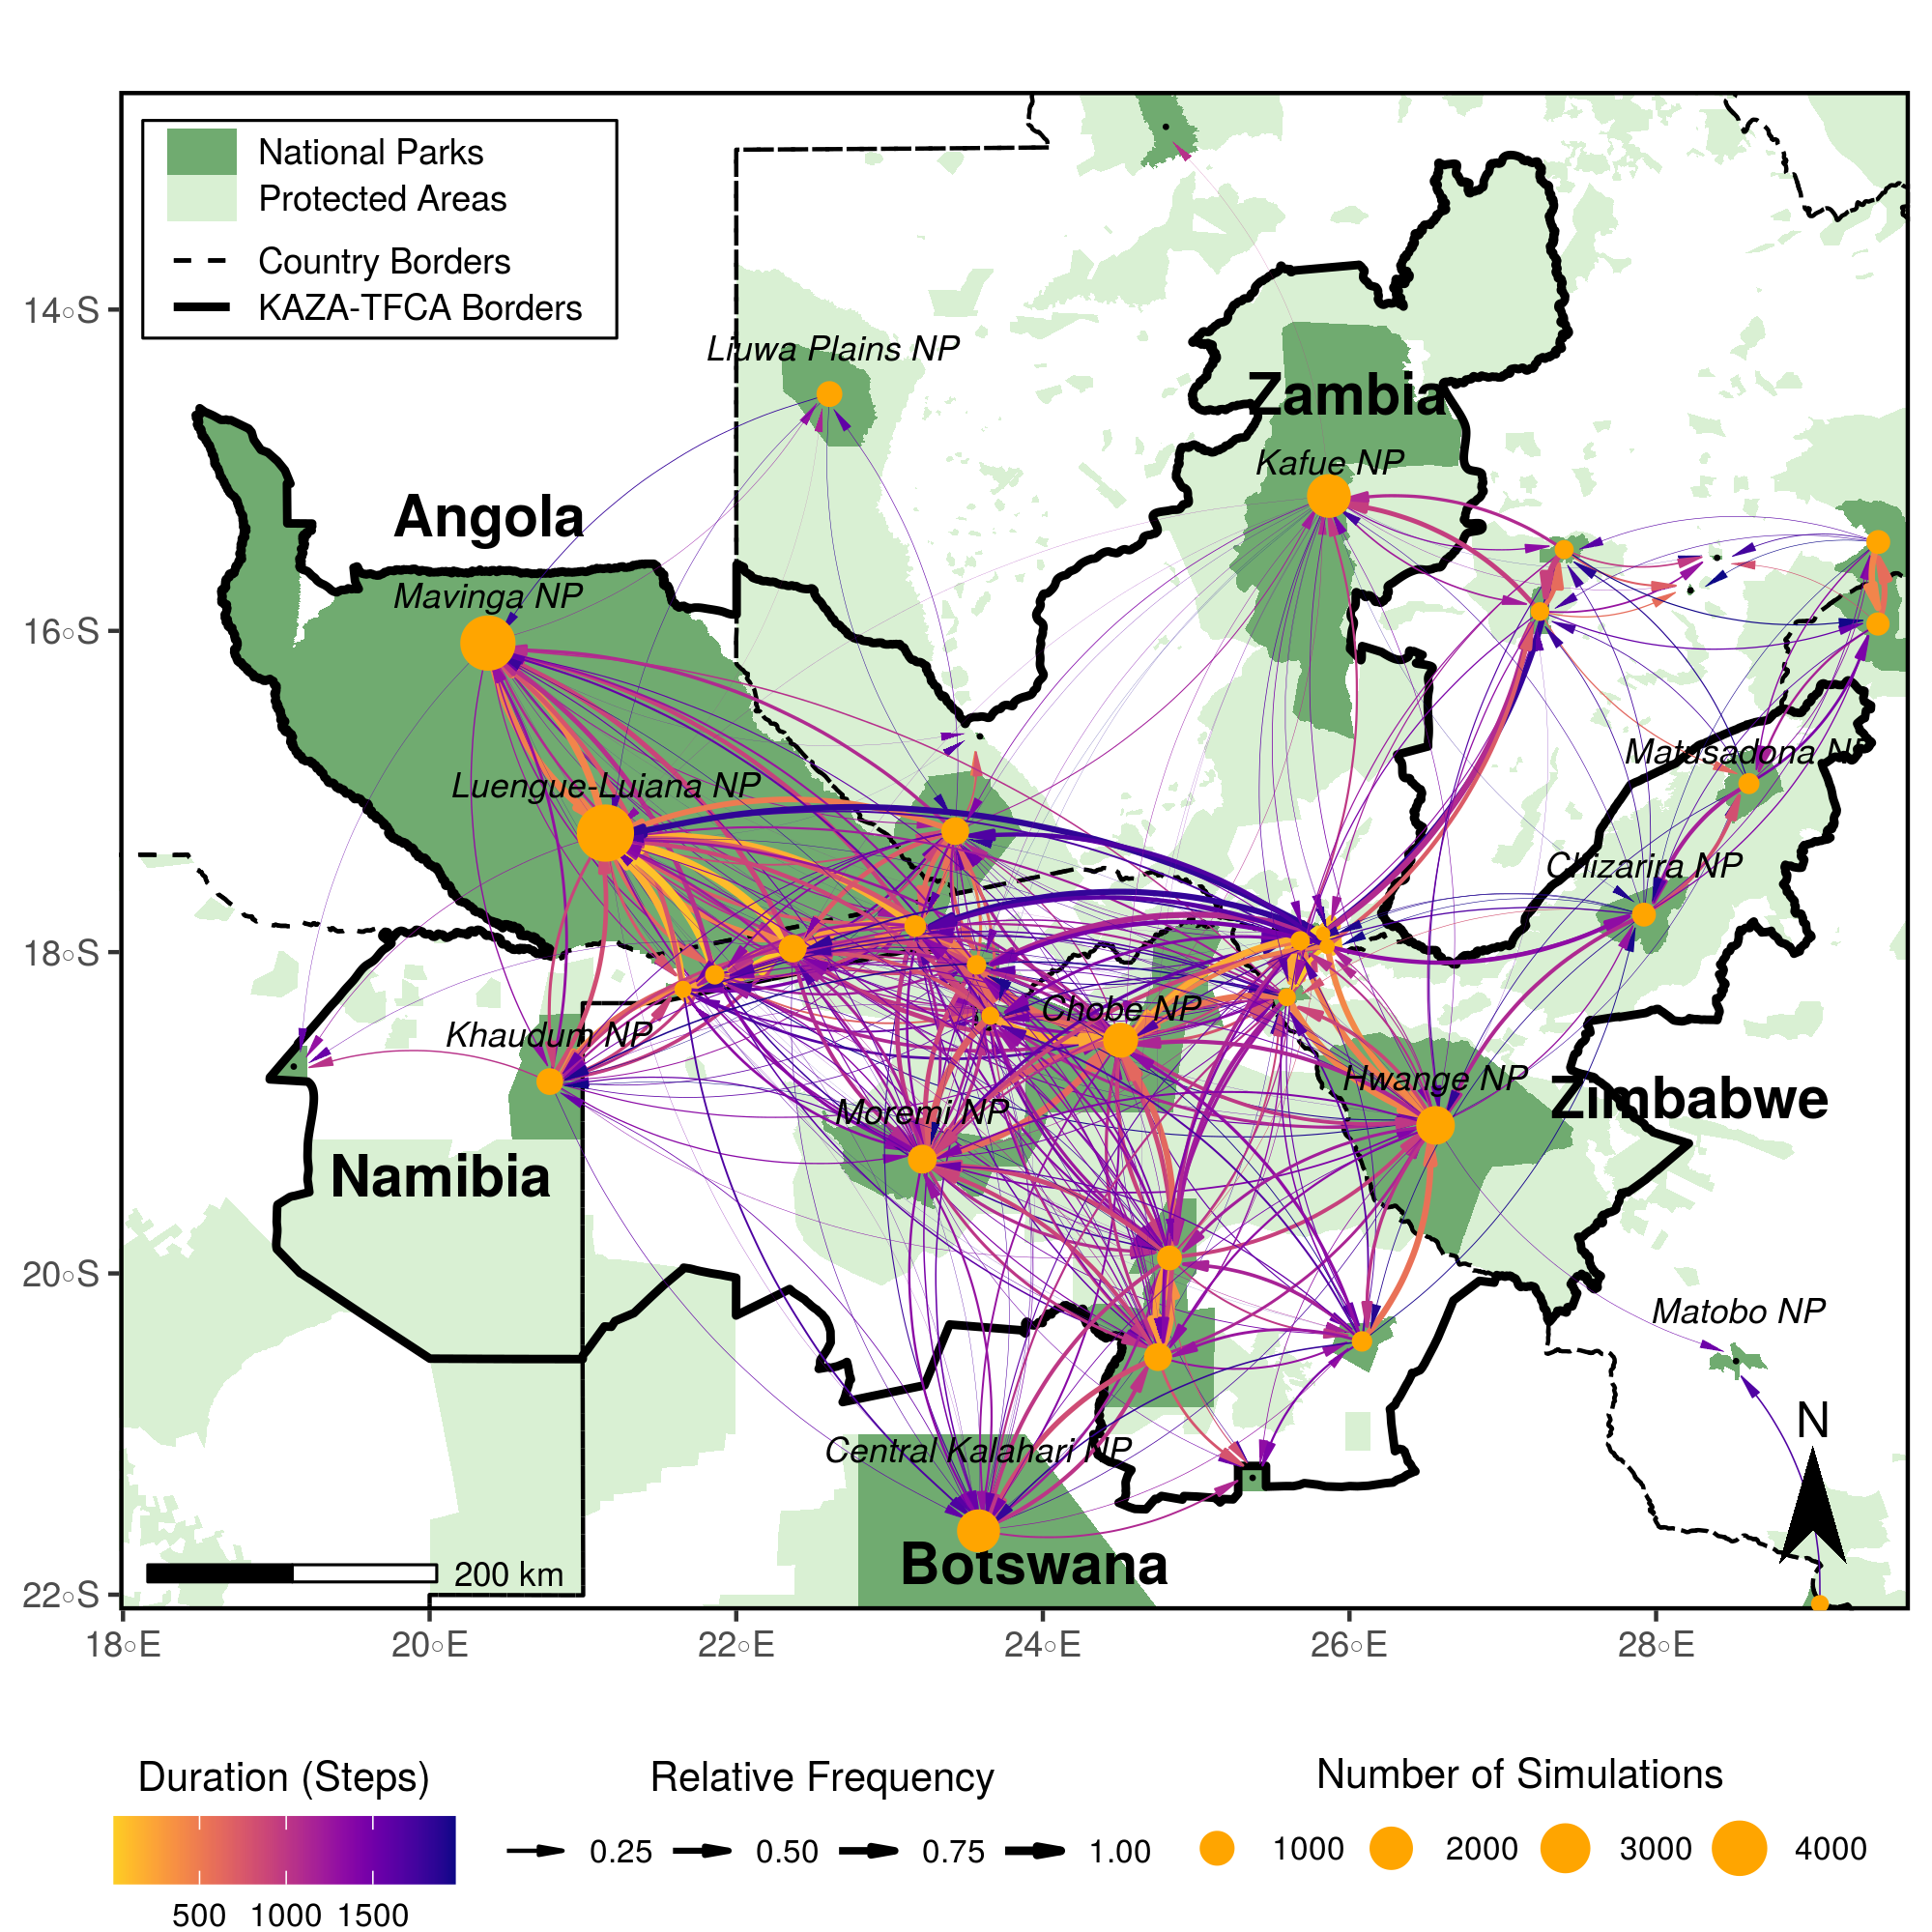
\includegraphics[width=\textwidth]{99_InterpatchConnectivity.png}
  \caption{Map of inter-patch connectivity in relation to dispersal duration,
  highlighting connections between NPs (dark green). Yellow bubbles represent
  the center of the different NPs and are sized in relation to the number of
  simulated dispersers originating from each park. Black dots represent NPs that
  were smaller than 700 km\textsuperscript{2} and therefore were not used as
  source areas. Arrows between NPs illustrate between which NPs the simulated
  dispersers successfully moved and the color of each arrow shows the average
  number of steps (i.e. 4-hourly movements) that were necessary to realize those
  connections. Additionally, the line thickness indicates the relative number of
  dispersers originating from a NP that realized those connections.}
  \label{InterpatchConnectivity}
\end{figure}

\section{Discussion}

% Short Summary
% \subsection{Short Summary}
Here, we presented a simple three-step approach to assess landscape connectivity
via simulated dispersal trajectories and we demonstrated its application using
empirical data from a free-ranging population of African wild dogs. In step one,
we used ISSFs to parametrize a fully mechanistic movement model describing how
individuals move through the landscape. Aside from rendering habitat
preferences, the model also encapsulated movement preferences and potential
interactions between movement and habitat preferences. In step two, we employed
the movement model and simulated dispersal trajectories across the landscape. In
comparison to more traditional connectivity modeling techniques, such
simulations require fewer unrealistic assumptions about dispersal and enable the
derivation of multiple connectivity metrics. Hence, in step three, we translated
the simulated trajectories into three complementary connectivity maps, each
emphasizing a different aspect of landscape connectivity (e.g. frequently
traversed areas, critical dispersal corridors and bottlenecks, and the presence
and intensity of functional links between suitable patches).

% Movement Model
% \subsection{Movement Model}
Results on the habitat kernel from our model showed that dispersers avoided
areas dominated by humans and covered by water, but selected for regions with
open grassland in the vicinity to water bodies. This largely complied with
previous studies that investigated habitat selection by dispersing wild dogs
\citep{DaviesMostert.2012, Masenga.2016, Woodroffe.2019, Oneill.2020,
Hofmann.2021}. However, instead of merely generating insights on dispersers'
habitat preferences, the ISSF framework also permitted us to model several
additional complexities common to dispersal. For instance, by including the
interactions \textsf{cos(ta):sl} and \textsf{cos(ta):log(sl)}, we could
accommodate that dispersers exhibit turning angles that are correlated with step
lengths, meaning that turning angles tend to be smaller when individuals move
fast. Although similar autocorrelations could be incorporated by sampling step
lengths and turning angles from copula probability distributions
\citep{Hodel.2022}, the ISSF framework allowed us to conveniently model such
peculiarities directly in the movement model. While we only considered first
order autocorrelation, i.e. correlation between two consecutive steps, higher
order autocorrelation is conceivable and may be desirable to model
\citep{Dray.2010, McClintock.2012}. However, this will require vast amounts of
GPS data that are not interrupted by missing fixes; something that is rarely
achieved in reality \citep{Graves.2006}. The power and flexibility of ISSFs to
model additive effects between habitat and movement covariates
\citep{Avgar.2016, Signer.2017} furthermore allowed us to formally capture that
dispersing wild dogs move slower and more tortuous in areas covered by water.
Such effects may be of limited interest and novelty from a biological
perspective, yet they are important to be considered when simulating dispersal,
in particular if one is interested in estimating dispersal durations between
habitat patches. Overall, the inclusion of interactions between habitat and
movement covariates in our movement model lead to a significant improvement in
predictive performance compared to an earlier model that omitted such
interactions \citep{Hofmann.2021}.

% The model also enabled us to include the interaction \textsf{sl:LowActivity} to
% render that wild dogs primarily move at dask and dawn. The resulting beta
% estimate was large, demonstrating the necessity to consider different phases of
% activities of the focal species.

% \subsection{Maps}
Each of the three connectivity maps derived from simulated dispersal
trajectories highlighted a different aspect of landscape connectivity. The
heatmap was most suitable for pinpointing frequently traversed areas and showed
that an exceptionally large number of dispersers moved through the regions of
the Moremi NP and the Chobe NP in northern Botswana. \cite{Hofmann.2021}
previously identified the same area as potential dispersal hotspot using LCPA,
however, following their analysis it was not clear whether this was the
consequence of the central location of the region and connections being enforced
between predefined start and endpoints. Contrary to LCPA, a simulation-based
approach as presented here does not require predefined endpoints, as endpoints
emerge naturally from the simulated dispersal trajectories. This is especially
useful for dispersal studies, where known endpoints are usually an unrealistic
assumption \citep{Elliot.2014, Abrahms.2017, Cozzi.2020}. The fact that the same
region was emphasized using vastly different methods to model connectivity thus
reinforces our notion that the area is of exceptional importance to dispersing
wild dogs. Because simulated individuals are not forced to move towards certain
endpoints, a simulation-based approach not only lends itself to study landscape
connectivity, but also to uncover potential dispersal traps
\citep{VanDerMeer.2014} or areas with a high susceptibility for human wildlife
conflicts \citep{Cushman.2018}.

In contrast to the heatmap, the betweenness map emphasized relatively narrow and
linear movement routes. It thus facilitated the identification of discrete
movement corridors. While in some cases both the heatmap and the betweenness map
attributed a high importance to the same areas (e.g. northern Botswana), little
consensus was found for other regions. For instance, the stretch of unprotected
land between Luengue-Luiana NP in Angola and the Kafue NP in Zambia was
characterized by a high betweenness-scores, yet it only received low scores on
the heatmap. This is due to the differential way in which the maps view
connectivity. While the heatmap attributes a high connectivity to areas that are
frequently traversed, it does not distinguish between areas that truly bring
individuals into other regions of the study area and regions that lead into
ecological traps. The converse is true on the betweenness map, as it strictly
highlights regions that promote movement into other areas of the landscape and
thus promote gene-flow. However, neither of the two maps provides insights into
functional links between distinct habitat patches or how connections depend on
the dispersal duration. For this reason, we also produced a map of inter-patch
connectivity. This map depicted the frequency at which simulated individuals
moved between patches as well as the average dispersal duration (in steps)
required to realize them. Calculating dispersal durations was only possible
because trajectories were simulated spatially and temporally explicitly,
something that is currently unfeasible with LCPA or CT. An explicit
representation of time enables answerings questions such as: ``\textit{How long
will it take a disperser to move from A to B?}'' or ``\textit{Is it possible for
a disperser to move from A to B within X days?}''. Moreover, it yields
opportunities to incorporate seasonality and to investigate whether dispersal
corridors exist seasonally or all-year round (\textit{dynamic connectivity};
\citealp{Zeller.2020}). With LCPA or CT, seasonality can currently only be
incorporated through the preparation of multiple permeability surfaces on which
the same connectivity model is repeatedly applied (e.g. \citealp{Osipova.2019}).
With simulations from ISSFs, in contrast, the environment could change ``as the
dispersers move'', so that simulated trajectories would dynamically respond to
seasonal fluctuations in the environment.

% \subsection{Structural vs. Functional Connectivity}
% Our approach enabled us to translate a simple set of small-scale behavioral
% rules into large scale patterns of connectivity, something previously deemed
% computationally unfeasible, yet critical for linking structural to functional
% connectivity \citep{Doerr.2011}. Structural connectivity focuses purely on the
% spatial arrangement of suitable habitat in the landscape, whereas functional
% connectivity also takes into account a species dispersal ability and behavioral
% response to the landscape \citep{Tischendorf.2000}. Functional connectivity is
% of greater interest in conservation science, yet much more difficult to measure
% \citep{Baguette.2013}, which is why structural connectivity often serves as
% surrogate., by contrast, is easier to measure and contributes significantly to
% functional connectivity, which is why it often serves as surrogate for
% functional connectivity \cite{Doerr.2011, Fattebert.2015}. Through incorporation
% of a species habitat preferences into a permeability surface, both LCPA and CT
% allow

Our approach enabled us to translate a simple set of small-scale behavioral
rules into large scale patterns of connectivity, something previously deemed
computationally unfeasible, yet critical for linking structural and functional
connectivity \citep{Doerr.2011}. Structural connectivity focuses purely on the
spatial arrangement of suitable habitat in the landscape, whereas functional
connectivity also takes into account a species dispersal ability and behavioral
response to the landscape \citep{Tischendorf.2000}. Functional connectivity is
of greater interest to conservation scientists, yet is difficult to quantify
\citep{Baguette.2013}, which is why structural connectivity often serves as
surrogate \cite{Doerr.2011, Fattebert.2015}. LCPA and CT incorporate functional
aspects of connectivity through the permeability surface, which reflects a
species habitat preferences and thus renders behavioral impacts of the lanscape
on the focal species. Aside from rendering habitat preferences, our model also
integrates peculiarities of the focal species movement behavior, thus adding
further insights on functional connectivity. In addition, we could use
independent dispersal data to prove that our predictions of connectiviy aligned
with observed functional connectivity patterns.

% If I were to force a couple of comments it would be how the authors discussed
% the shift from a structural to a functional view on connectivity (lines 38-39).
% For one, using the integrative approach appears to me as a way where the
% movement and habitat kernels (and the interaction between them) inform the
% relationship between structural connectivity (the landscape) and functional
% connectivity (dispersal), which I believe is the core of the Tishendorf & Fahrig
% (2000) paper. Consequently, I don’t see this as a shift, but more an
% approximation to understand how they are related. Two, because understanding the
% relationship between structural and functional connectivity is a key goal in
% landscape ecology, I feel the authors could have discussed the implication of
% this approach to this end.

% \subsection{Disadvantages of ISSF Simulations}
Despite the many benefits and great flexibility offered by simulations from
ISSFs, one must also be aware of the associated limitations. For example, while
our approach of simulating dispersal proved usedful to assess landscape
connectivity, it was computationally costly. Simulating 80,000 dispersal
trajectories for 2'000 steps across the KAZA-TFCA required five days of
computation on a regular desktop machine (AMD Ryzen 7 2700X octa-core processor
with 3.6 GHz, 64 GB of RAM). The long simulation time was primarily caused by
the massive extent of the study area considered (ca. 1.8 Mio
km\textsuperscript{2}), the large number of simulated trajectories, and the fact
that we extracted covariates along each step, rather than just at their start or
endpoints. Most connectivity studies focus on smaller study areas (e.g.
\citealp{Kanagaraj.2013, Clark.2015, McClure.2016, Abrahms.2017, Zeller.2020})
and will therefore require fewer simulations and achieve faster simulation times
(given the same spatial resolution). We also believe that fewer simulated
trajectories will often suffice, as the relative traversal frequency by
simulated trajectories through randomly placed checkpoints across our study area
converged already after 10,500 runs. The exact number of required simulations to
achieve reliable estimates of connectivity will, of course, vary depending on
the structure of the landscape and the dispersal capabilities of the focal
species \citep{Gustafson.1996}. For species that disperse short distances
through homogeneous environments, few simulations may suffice to gauge
connectivity, whereas for species that disperse over long distances through
heterogeneous habitats, a large number of simulations will be required to
sufficiently explore the spectrum of possible routes. Finally, it may often
suffice to extract covariates at each step's start or endpoints, thus
considerably speeding up simulation times \citep{Signer.2017}.

Aside from the computational requirements, simulations further entail several
non-trivial but important modeling decisions. On four such decisions we would
like to further elaborate: (1) the number of simulated individuals, (2) the
location of source points, (3) the simulated dispersal duration, and (4)
the behavior at map boundaries.

(1) When simulating dispersal trajectories, the modeler needs to decide on the
number of simulated individuals. A higher number is always desirable, as each
additional trajectory provides information about landscape connectivity.
However, each additional simulation imposes computational costs, so a trade-off
needs to be managed. \cite{Signer.2017} proposed to handle the trade-off by
simulating additional individuals only until the metrics of interest converge
towards a steady state. Here, we used the relative traversal frequency as target
metric and found that it converged already after 10'500 simulated individuals.
The exact number of required individuals might, however, vary depending on the
employed target metric and the anticipated connectivity map. More sophisticated
target metrics than the relative traversal frequency, preferably tailored to
different connectivity maps, need to be developed in the future.

(2) To initiate dispersers, a modeler needs to provide a set of source points at
which the virtual dispersers are released. We placed source points within
protected areas large enough to sustain viable wild dog populations, implicitly
assuming that wild dogs primarily survive in large, formally protected areas
\citep{DaviesMostert.2012, Woodroffe.2012, VanDerMeer.2014}. Moreover, we lacked
precise knowledge about the distribution and abundance of wild dogs across
protected areas, so we placed source points randomly within them. In cases where
more detailed data about the distribution and abundance of the focal species are
available, source points could be distributed accordingly. Alternatively, source
points could be distributed homogeneously but later be weighted when computing
connectivity metrics. In any case, the challenge of selecting meaningful source
points is not unique to individual-based simulations but also applies to LCPA
and CT.

(3) The use of ISSFs to simulate dispersers requires deciding on the number of
simulated steps (i.e. the simulated dispersal durations). If sufficient
dispersal data of the focal species has been collected, dispersal durations
could be sampled from observed dispersal events or from parametric distributions
fit to observed data. Due to the low number of observed dispersal events, we
opted against this solution and instead simulated all individuals for 2,000
steps, which was at the upper end of observed dispersal durations in African
wild dogs \citep{DaviesMostert.2012, Masenga.2016, Cozzi.2020, Hofmann.2021}.
This approach had the advantage that it allowed us to systematically shorten the
simulated trajectories after their simulation and thereby to investigate the
sensitivity of our results with respect to exact dispersal durations (Figures S5
and S6).

(4) Unless simulated dispersal trajectories are strongly drawn towards a point
of attraction inside the study area(e.g. \citealp{Signer.2017}), some
trajectories will inevitably approach one of the map boundaries. In this case,
one or more of the generated random steps might leave the study area, making it
impossible to compute a selection score. A possible solution is to simply
terminate the simulation of the affected trajectory, assuming that the simulated
individual has left the study area. However, this approach might produce
ambiguous results in cases where many individuals are released near map borders,
especially because already a single random step leaving the study area will
break the simulation, thus resulting in biased connectivity estimates along map
borders. Rather than breaking the simulation, we created a buffer zone
\citep{Koen.2010} and resampled random steps until they fully lied within the
study area. This proved to be an effective solution to overcome problems with
boundary effects.

% \subsection{Conclusion}
In summary, we proposed and applied a simple three-step approach that relies on
ISSF-analysis and enables the simulation of dispersal trajectories and the
assessment of landscape connectivity. The proposed approach overcomes several of
the conceptual shortcomings inherent to LCPA and CT, such as the assumption of
known endpoints, and provides a highly flexible tool for investigating
connectivity. Moreover, the simulation of dispersal opens up new avenues for
incorporating interactions between habitat and movement covariates and provides
the foundation for a rich suite of complementary connectivity measures. With
this work, we hope to have sparked interest in the application, optimization, or
creation of methods to investigate dispersal and connectivity via
individual-based simulations, while at the same time stressing some of the
non-trivial modeling decisions involved. We also hope to provide a useful
framework that helps unifying and streamlining the application of
individual-based simulations for assessing landscape connectivity.

\section{Authors' Contributions}
D.D.H., D.M.B., A.O. and G.C. conceived the study and designed methodology;
D.M.B., G.C., and J.W.M. collected the data; D.D.H. and D.M.B. analysed the
data; G.C. and A.O. assisted with modeling; D.D.H., D.M.B., and G.C. wrote the
first draft of the manuscript and all authors contributed to the drafts at
several stages and gave final approval for publication.

\section{Data Availability}
GPS movement data of dispersing wild dogs is available on dryad
\citep{Hofmann.2021b}. Access to R-scripts that exemplify the application of the
proposed approach using simulated data are provided through Github
(\url{https://github.com/DavidDHofmann/DispersalSimulation}). In addition, all
codes required to reproduce the African wild dog case study will be made
available through an online repository at the time of publication.

\section{Acknowledgements}
We thank the Ministry of Environment and Tourism of Botswana for granting
permission to conduct this research. We thank C. Botes, I. Clavadetscher, and G.
Camenisch for assisting with wild dog immobilizations. We also thank B. Abrahms
for sharing her data of three dispersing wild dogs. Furthermore, we would like
to thank Johannes Signer for assisting with the simulation algorithm. This study
was funded by Albert-Heim Foundation, Basler Stiftung für Biologische Forschung,
Claraz Foundation, Idea Wild, Jacot Foundation, National Geographic Society,
Parrotia Stiftung, Stiftung Temperatio, Wilderness Wildlife Trust,
Forschungskredit of the University of Zürich (grant no. FK-21-091), and a Swiss
National Science Foundation grant (no. 31003A\_182286) to A. Ozgul.

\section{Conflict of Interest}
All authors declare that they have no conflicts of interest.

\newpage
\begingroup
\singlespacing
\bibliography{Literatur}
\endgroup

\end{document}
